\documentclass{styles/diploma/diploma}
%\usepackage[backend=biber]{biblatex}
\addbibresource{main.bib}

\begin{document}

%\part{title}
\student{Трофимов Владислав Олегович}
\group{М8О-403Б-21}
\theme{Разработка системы тематической кластеризации научных работ на основе семантического подхода  с визуализацией в графовом интерфейсе}

\supervisor{Кан Анна Владимировна}
\secondConsultant{---}
\reviewer{---}

\faculty{№ 8 <<Компьютерные науки и прикладная математика>>}
\department{805}
\speciality{01.03.04 <<Прикладная математика>>}
\profile{Математическое и программное обеспечение систем обработки информации и управления}

\departmentFullName{№ 805}
\headOfDepartment{Пантелеев Андрей Владимирович}

% Дата. Оставляем пустое место для дня
\date{\uline{\hspace{24pt}} мая \the\year\ года}

\newacronym{amqp}{AMQP}{advanced message queuing protocol}
\newacronym{api}{API}{application programming interface}
\newacronym{cicd}{CI/CD}{continuous integration/continuous deployment}
\newacronym{esc}{ESC}{elastic container service}
\newacronym{gil}{GIL}{global interpreter lock}
\newacronym{grpc}{gRPC}{google remote procedure calls}
\newacronym{mse}{MSE}{mean squared deviation}
\newacronym{mvp}{MVP}{minimum viable product}
\newacronym{mqtt}{MQTT}{message queuing telemetry transport}
\newacronym{rest}{REST}{representational state transfer}
\newacronym{stomp}{STOMP}{streaming text oriented messaging protocol}
\newacronym{субд}{СУБД}{система управления базами данных}
\newacronym{яп}{ЯП}{язык программирования}
\newglossaryentry{id1}{ % Нужны разные id, можно ставить просто последовательно
    name={\LaTeX},
    description={система компьютерной вёрстки} 
}
\newglossaryentry{id2}{
    name={МАИ},
    description={Московский Авиационный Институт} 
}
\newglossaryentry{id3}{
    name={$S^{2}$},
    description={формула в списке обозначений} 
}


% Иллюстрации всегда по центру
\makeatletter
\g@addto@macro\@floatboxreset\centering
\makeatother

\maketitle

% \includepdf[pages=-]{extra/task} % Задание
\setcounter{page}{2} % Устанавливает счётчик страниц

\abstract % Структурный элемент: РЕФЕРАТ

\keywords{КЛАСТЕРИЗАЦИЯ, СЕМАНТИЧЕСКИЙ АНАЛИЗ, МИКРОСЕРВИСЫ, HDBSCAN, SBERT, PostgreSQL, RABBITMQ, ГРАФОВЫЙ ИНТЕРФЕЙС}

В работе разработана и реализована высокопроизводительная система кластеризации документов, принимающая файлы форматов PDF и DOCX, которая генерирует кластеры из извлечённых текстовых данных и визуализирует результаты в графовом интерфейсе.

Практическая часть включает разработку приложения, построенного на микросервисной архитектуре, которая обеспечивает гибкость, масштабируемость и изоляцию компонентов. Система состоит из следующих компонентов: хранилище данных (S3), брокер сообщений (RabbitMQ), база данных (PostgreSQL), сервисы Public API и Clustulizer, а также пользовательский интерфейс.

Public API реализован на языке Golang с использованием фреймворка Fiber и обеспечивает обработку HTTP-запросов пользователей. Сервис Clustulizer реализован на Python, использует модель SBERT-LARGE-NLU-RU для генерации эмбеддингов и алгоритм кластеризации HDBSCAN.

Оценка качества кластеризации показала высокий уровень с использованием метрик Silhouette Score (0.923) и низкий индекс Davies-Bouldin (0.107), подтверждая эффективность предложенного решения. Среднее время обработки документов составляет 120 мс, с пропускной способностью до 40 документов в секунду.

Пользовательский интерфейс системы обеспечивает наглядное представление результатов в виде интерактивного графа, позволяя пользователям легко ориентироваться в результатах обработки. % Реферат

\tableofcontents % Содержание 
% \termsanddefenitions % Термины и определения
%\listofabbreviations % Перечень сокращений и обозначений
 
\introduction % Структурный элемент: ВВЕДЕНИЕ
Постоянный и впечатляющий прогресс в области компьютерного оборудования за последние годы привёл к широкому распространению мощных и доступных компьютеров, средств сбора данных и устройств хранения информации. Благодаря этому прогрессу индустрия баз данных и информационных технологий получила мощный импульс для создания огромного количества баз данных и информационных хранилищ, которые используются для управления транзакциями, поиска информации и анализа данных.

Таким образом, технологическое развитие обеспечило стремительный рост объёма текстовых документов, доступных в интернете, цифровых библиотеках и репозиториях, новостных источниках, корпоративных интрасетях и оцифрованной личной информации, такой как блоги и электронные письма. С увеличением количества электронных документов становится всё сложнее вручную их организовывать, анализировать и представлять эффективно. Это породило вызовы в сфере эффективной автоматической организации текстовых документов.

Решение данной проблемы связано с применением передовых технологий, таких как машинное обучение, искусственный интеллект и методы кластерного анализа. Эти методы позволяют автоматизировать процессы организации информации, повышая скорость обработки данных, точность результатов и удобство их последующего использования.





% ------
% С быстрым развитием цифровых технологий доступ к информации стал более распространённым аспектом повседневной жизни, чем когда-либо прежде. Бизнес и частные лица теперь имеют доступ к огромному объёму данных — миллиардам документов, видео- и аудиофайлов в интернете. Большинство компаний функционируют в тесно взаимосвязанной среде данных, связанной с множеством информационных источников, что позволяет получать доступ к значительным объёмам информации. Однако, несмотря на быстрый рост вычислительных возможностей, сам по себе огромный объём данных часто затрудняет преобразование разрозненной информации в полезные сведения, практические знания и конкретные действия. Одним из устоявшихся решений является использование машинного обучения, в частности методов кластеризации.

% Алгоритмы кластеризации — это алгоритмы машинного обучения, которые стремятся группировать схожие данные на основе определённых критериев, выявляя тем самым естественные структуры или закономерности в наборе данных. Основная цель — разделить данные на подгруппы (кластеры), элементы которых внутри одного кластера более похожи друг на друга, чем на элементы других кластеров. Методы кластеризации способствуют развитию различных областей, таких как поиск информации, рекомендательные системы и выявление тем.

% Алгоритмы кластеризации широко применяются в повседневной жизни. Их используют для фильтрации спама, в рекомендательных системах, для сегментации клиентов в целях таргетированного маркетинга, в обработке изображений — для группировки изображений по визуальному сходству и многого другого. Алгоритмы кластеризации применимы как к текстовым данным, так и к аудио-, видео- и графическим материалам. Аудиокластеризация использует акустические характеристики для группировки файлов и может применяться, например, для определения музыкальных жанров. Кластеризация видео помогает в создании рекомендаций и аннотаций, группируя контент по визуальным или тематическим признакам. В анализе изображений кластеризация важна для сегментации и поиска по содержанию. Алгоритмы кластеризации также используются для выявления аномалий — будь то в сетевом трафике, финансовых транзакциях или медицинских записях. Их универсальность подчёркивает значимость этих алгоритмов в выявлении закономерностей из самых разных типов данных.
% Два основных типа алгоритмов кластеризации, исходя из наличия размеченных данных и способа обучения, следующие:
% \begin{itemize}[label=., leftmargin=3em]
%     \item Полу-контролируемая кластеризация (Semi-supervised Clustering):
    
% В этой категории для каждой обучающей выборки предоставляется известная метка кластера. Алгоритм анализирует закономерности в обучающих данных и затем учится присваивать новые точки данных соответствующим кластерам. Примеры таких алгоритмов включают Constrained K-Means [1] и Semi-Supervised Fuzzy C-Means (SSFCM)

%     \item Ненаблюдаемое (без учителя) обучение (Unsupervised Learning):
    
% В этой категории метки классов (кластеров) не предоставляются. Алгоритм самостоятельно выявляет закономерности и структуры в данных, группируя похожие образцы на основе сходства признаков без предварительного знания о принадлежности к группам. Обычно общее количество кластеров в наборе данных заранее неизвестно. Примеры алгоритмов в этой категории включают K-Means [3, 4], DBSCAN (Density-Based Spatial Clustering of Applications with Noise) [5] и Fuzzy C-Means (FCM) [6].
% \end{itemize}


% Для определения подходящего количества кластеров могут использоваться различные методы, такие как метод локтя (elbow method), коэффициент силуэта (silhouette score), статистика разрыва (gap statistics) 
 % Введение

\teory % Структурный элемент: ТЕОРИЯ

Кластеризация (или кластерный анализ) — это задача разбиения множества объектов на группы, называемые кластерами. Внутри каждой группы должны оказаться «похожие» объекты, а объекты разных группы должны быть как можно более отличны. Главное отличие кластеризации от классификации состоит в том, что перечень групп четко не задан и определяется в процессе работы алгоритма
Применение кластеризация в общем виде сводится к следующим этапам:
\begin{enumerate}[label=\arabic*.]
\item Отбор выборки объектов для кластеризации.

\item Определение множества переменных, по которым будут оцениваться объекты в выборке. При необходимости – нормализация значений переменных.

\item Вычисление значений меры сходства между объектами.

\item Применение метода кластерного анализа для создания групп сходных объектов (кластеров).
	
\item Представление результатов анализа
		
	\end{enumerate}

Кластеризация может быть либо непересекающейся (жёсткой), либо пересекающейся. В пересекающейся кластеризации один и тот же документ может принадлежать к нескольким кластерам, в то время как при жёсткой кластеризации каждый документ попадает только в один кластер.

Кластеризация отличается от классификации документов. В классификации классы (и их характеристики) известны заранее, и документы просто распределяются по этим классам. В кластеризации количество, свойства и состав классов заранее неизвестны. Таким образом, классификация — это пример обучения с учителем, а кластеризация — обучения без учителя.

Кластеризация документов делится на две основные подкатегории: жёсткая (hard clustering) и мягкая (soft clustering). Мягкая кластеризация, также известная как пересекающаяся, далее подразделяется на:

    

\begin{itemize}
    \item Жёсткая кластеризация:
    Каждый документ жёстко назначается одному кластеру — формируются непересекающиеся кластеры;

    \item Мягкая кластеризация (Soft/Overlapping):
    Документ может входить сразу в несколько кластеров. Например, документ о «естественном языке и информационном поиске» может быть отнесён к обоим кластерам — «Естественный язык» и «Информационный поиск»;
     \item Разделяющая кластеризация (Partitioning):
    Делит документы на фиксированное количество непустых кластеров. Самый известный метод — K-средних (K-means) и его варианты [4]. Алгоритм начинается с случайного распределения объектов по кластерам, затем в каждой итерации пересчитываются центры (средние) кластеров, и объекты перераспределяются по ближайшим центрам. Алгоритм завершается, когда перераспределение прекращается;
     \item Иерархическая кластеризация (Hierarchical)
    Строит дендрограмму — дерево кластеров, где листья — подмножества документов. Примеры: Иерархическая агломеративная кластеризация (HAC) и метод UPGMA;
     \item Кластеризация на основе частых наборов признаков (Frequent itemset-based):
   Эти методы используют часто встречающиеся наборы признаков (itemsets), извлечённые с помощью ассоциативных правил, для кластеризации документов. Это снижает размерность признаков и улучшает точность и масштабируемость алгоритмов. Дополнительно, каждый кластер можно обозначить частыми наборами терминов.
\end{itemize}


   
В этой категории метки классов (кластеров) не предоставляются. Алгоритм самостоятельно выявляет закономерности и структуры в данных, группируя похожие образцы на основе сходства признаков без предварительного знания о принадлежности к группам. Обычно общее количество кластеров в наборе данных заранее неизвестно. Примеры алгоритмов в этой категории включают K-Means, DBSCAN (Density-Based Spatial Clustering of Applications with Noise) и Fuzzy C-Means (FCM).


Изначально кластеризация документов изучалась с целью повышения точности и полноты (precision и recall) в системах информационного поиска. Также кластеризация используется для автоматического построения иерархических кластеров документов.
Существуют основные сферы применения кластеризации данных:
\begin{itemize}
   \item \textbf{Обнаружение тем (Topic Discovery)}:
       Позволяет выявить скрытые темы и тенденции в больших коллекциях документов;
    \item \textbf{Автоматическая организация контента}:
       Используется для структурирования и классификации информации в новостных сайтах, блогах, корпоративных порталах и цифровых библиотеках;
    \item \textbf{Информационный поиск (Information Retrieval)}:
       Кластеризация помогает группировать документы по темам, повышая релевантность выдачи и упрощая пользователям поиск нужной информации;
    \item \textbf{Мягкая кластеризация (Soft/Overlapping)}:
        Документ может входить сразу в несколько кластеров. Например, документ о «естественном языке и информационном поиске» может быть отнесён к обоим кластерам — «Естественный язык» и «Информационный поиск»;
    \item \textbf{Рекомендательные системы}:
    Позволяет выявить скрытые темы и тенденции в больших коллекциях документов.  ;
    \item \textbf{Автоматическая организация контента}:
       Кластеры документов могут быть использованы для создания кратких тематических сводок;
    \item \textbf{Анализ мнений и отзывов}:
    Помогает в группировке отзывов пользователей по схожим аспектам или эмоциональной окраске;
    \item \textbf{Управление знаниями (Knowledge Management)}:
    В корпоративных системах — для организации внутренних документов, отчетов и технической документации.
\end{itemize}
\section{Алгоритмы кластеризации}
    
\subsection{K MEANS}

Это один из самых популярных методов кластеризации, используемых в машинном обучении. В отличие от обучения с учителем, обучающие данные, которые использует этот алгоритм, не размечены, то есть точки данных не имеют заранее определённой структуры классификации.

Существует множество типов алгоритмов кластеризации, включая эксклюзивную, перекрывающуюся, иерархическую и вероятностную. Алгоритм кластеризации k-средних (k-means) является примером эксклюзивной или «жёсткой» кластеризации. Такая форма группировки предполагает, что каждая точка данных может принадлежать только одному кластеру. Этот тип кластерного анализа широко применяется в области анализа данных для сегментации рынка, кластеризации документов, сегментации изображений и сжатия изображений. Алгоритм k-средних популярен благодаря своей эффективности, простоте и высокой производительности.

Алгоритм k-средних — это итеративный алгоритм кластеризации, основанный на центроидах. Он разбивает набор данных на группы по признаку схожести, определяемой расстоянием до центроида. Центроид (или центр кластера) представляет собой среднее или медианное значение всех точек в кластере — в зависимости от характеристик данных.

Кластеризация методом k-средних представляет собой итеративный процесс минимизации суммы расстояний между точками данных и центроидами соответствующих кластеров.

\begin{equation}
V = \sum_{i=1}^{k} \sum_{x \in S_i} (x - \mu_i)^2,
\end{equation}

где:
\begin{itemize}

\item $k$ — число кластеров;
\item $S_i$ — полученные кластеры;
\item $i = 1,2,\ldots$;
\item $\mu_i$ — центры масс всех векторов из кластера.
\end{itemize}


Алгоритм кластеризации k-средних работает путём категоризации точек данных в кластеры на основе математической меры расстояния — обычно евклидовой — до центра кластера. Цель — минимизировать сумму расстояний между точками данных и их соответствующими центроидами. Точки данных, ближайшие к центроиду, группируются в одну категорию. Более высокое значение k (число кластеров) означает меньшие по размеру, но более детализированные кластеры; более низкое значение k — более крупные кластеры с меньшей детализацией.

Следующий шаг включает в себя двухэтапный итерационный процесс, основанный на алгоритме машинного обучения ожидания-максимизации. На этапе ожидания каждая точка данных присваивается ближайшему центроиду на основе расстояния (обычно евклидова). На этапе максимизации вычисляется среднее значение всех точек для каждого кластера и пересчитывается центр кластера — центроид. Этот процесс повторяется до тех пор, пока положения центроидов не стабилизируются (сойдутся) или не будет достигнуто максимальное количество итераций.

Алгоритм кластеризации K-средних прост, но чувствителен к начальным условиям и выбросам. Важно оптимизировать инициализацию центроидов и количество кластеров k, чтобы получить максимально информативные кластеры. 

Ввиду этого я выбрал более подходящих алгоритм кластеризации в своей работает - HDBSCAN.

\subsection{HDBSCAN}
HDBSCAN основан на DBSCAN, поэтому стоит рассказать сначала о нем.

Алгоритм DBSCAN — это классический метод кластеризации на основе плотности, который эффективно определяет шумовые (выбросные) точки. Он рассматривает кластеры как наибольшие множества данных, связанных плотностью, и основным принципом является то, что точки, принадлежащие одному кластеру, связаны друг с другом через плотность.

Алгоритм DBSCAN был впервые предложен Эстером и соавторами. Каждая точка данных в кластере должна иметь в своём окрестности (радиусе Eps) как минимум заданное количество точек (MinPts). 

Алгоритм DBSCAN использует итерационные запросы для выполнения кластеризации. Сначала, на основе заданных параметров Eps и MinPts, определяется множество всех основных (ядровых) точек в наборе данных — оно называется множеством N. Затем рассматривается основная точка o из набора данных. Если точка o ещё не отнесена к какому-либо кластеру, создаётся новый кластер C, и все точки в окрестности точки o, включая её саму, помечаются как принадлежащие кластеру C.

Далее, если некоторая точка p из окрестности o также является основной, то все точки в её окрестности также добавляются в кластер C. Эти действия повторяются для оставшихся точек кластера C, пока не перестанут добавляться новые точки. Описанный процесс повторяется для всех точек из множества N, которые ещё не были обработаны, до тех пор, пока все основные точки не будут рассмотрены.

Алгоритм DBSCAN последовательно «поглощает» точки, которые находятся в области плотности, напрямую доступной из основной точки p. Если между двумя кластерами существует плотностная связь, они объединяются в один. Это даёт преимущество в обнаружении кластеров произвольной формы и идентификации шумовых точек. Однако, производительность алгоритма по времени может быть низкой из-за необходимости нахождения основных точек и анализа всех остальных.
\begin{figure}[h!]
    \centering
    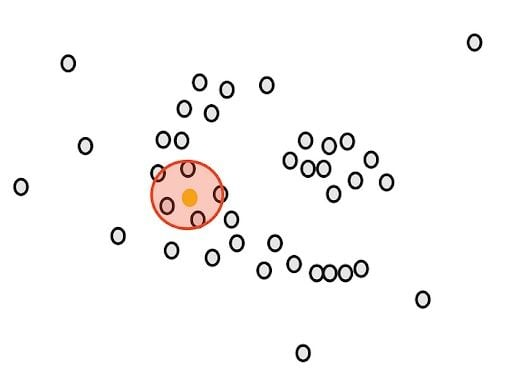
\includegraphics[width=0.7\textwidth]{styles/diploma/inc/dbscan.jpg} % можно .png, .pdf и т.п.
    \caption{Иллюстарция работы алгоритма DBSCAN}
    \label{fig:example}
\end{figure}

В свою очередь отличительным признаком  HDBSCAN является то, что он не выбирает кластеры на основе глобального порога epsilon, а создаёт иерархию для всех возможных значений epsilon с учётом параметра minPts как минимального размера кластера.
\subsubsection{Расстояние взаимной достижимости}
В HDBSCAN ядровое расстояние (dcore) определяется как расстояние от объекта до его minPts-ближайшего соседа. Построенная иерархия основана на взаимном достижимом расстоянии, которое для двух объектов $x_p$ и $x_q$ определяется как:

\begin{equation}
\max\{d_{\text{core}}(x_p),\ d_{\text{core}}(x_q),\ d(x_p, x_q)\} ,
\end{equation}
где:
\begin{itemize}
\item  $d(x_p, x_q)$ — обычное расстояние между объектами, например, евклидово. 
\end{itemize}

Такой подход отделяет разреженные точки от остальных хотя бы на их ядровое расстояние и делает кластеризацию устойчивее к шуму.





Набор данных можно представить в виде графа, где объекты — это вершины, соединённые рёбрами с весами, равными взаимному достижимому расстоянию. Построив по этому графу минимальное остовное дерево и отсортировав его рёбра по mutual reachability, формируется иерархическое дерево (дендрограмма). Задав значение epsilon как уровень горизонтального сечения и выбрав все кластеры, содержащие не менее minPts точек на этом уровне плотности, можно извлечь кластеры DBSCAN для этого epsilon из иерархии.

\subsubsection{Сжатая иерархия кластеров}

Поскольку HDBSCAN направлен на обнаружение кластеров с различной плотностью, он строит упрощённую версию сложного иерархического дерева — сжатое дерево кластеров. Этот подход следует концепции обрезки дерева, которая имеет много вариантов в литературе, таких как обрезка мелких кластеров (runt pruning) по Штюцле или обрезка дерева, построенного с помощью устойчивого алгоритма одиночной связи по Чаудхури и др.

Начиная с корня, HDBSCAN рассматривает разделение кластера как истинное только в том случае, если оба дочерних кластера содержат не менее minPts объектов. Если оба содержат меньше minPts, считается, что кластер исчез на этом уровне плотности. Если только один из дочерних кластеров содержит меньше minPts, считается, что родительский кластер просто потерял точки, но всё ещё существует. "Потерянные" точки считаются шумом. Этот процесс упрощения приводит к иерархии возможных кластеров на разных уровнях плотности.


\subsubsection{Выбор кластеров на основе стабильности}

Имея сжатое дерево кластеров, один из возможных подходов — просто выбрать все листовые узлы. Это кластеры с наименьшими значениями epsilon в иерархии, которые больше нельзя разделить с учётом параметра minPts. Этот метод выбора — один из двух вариантов, реализованных в Python-библиотеке HDBSCAN, и далее будет называться HDBSCAN(leaf). Он приводит к формированию мелких, детализированных кластеров.

Имея сжатое дерево кластеров, один из возможных подходов — просто выбрать все листовые узлы. Это кластеры с наименьшими значениями epsilon в иерархии, которые больше нельзя разделить с учётом параметра minPts. Этот метод выбора — один из двух вариантов, реализованных в Python-библиотеке HDBSCAN, и далее будет называться HDBSCAN(leaf). Он приводит к формированию мелких, детализированных кластеров.

Второй вариант — метод eom (excess of mass, избыток массы). Этот метод рекомендуется Кампелло и др. как оптимальное глобальное решение задачи выбора кластеров с наибольшей стабильностью. Он определяет стабильность следующим образом:
\begin{equation}
\begin{aligned}
S(C_i) &= \sum_{x_j \in C_i} \left( \lambda_{\max}(x_j, C_i) - \lambda_{\min}(C_i) \right) \\
       &= \sum_{x_j \in C_i} \left( \frac{1}{\varepsilon_{\min}(x_j, C_i)} - \frac{1}{\varepsilon_{\max}(C_i)} \right)
\end{aligned}
\end{equation}


Значение плотности $\lambda$ при этом принимается равным $\frac{1}{\epsilon}$. Это означает, что значения $\lambda$ возрастают от корня к листьям дерева, в то время как соответствующие значения расстояния $\epsilon$ уменьшаются. Вычитание $\lambda_{min}(C_i)$ — плотностного уровня, на котором кластер $C_i$ впервые появляется, из значения, при котором объект $x_j ∈ C_i$ больше не принадлежит $C_i$, даёт время жизни объекта $x_j$ в кластере. Суммируя времена жизни всех объектов в кластере $C_i$, получают общее время жизни кластера $S(C_i)$, которое называется стабильностью, поскольку кластеры с наибольшим временем жизни считаются наиболее устойчивыми.

Затем формируется задача оптимизации, целью которой является максимизация суммы стабильностей кластеров:
\begin{equation}
\begin{aligned}
\max_{\delta_2, \ldots, \delta_k} \quad & J = \sum_{i=2}^{k} \delta_i S(C_i) \\
\text{subject to} \quad & \delta_i \in \{0,1\}, \quad i = 2, \ldots, k \\
& \sum_{j \in I_h} \delta_j = 1, \quad \forall h \in \mathbf{L}
\end{aligned}
\end{equation}


где:
\begin{itemize}
    \item $L = \{h \mid C_h \text{ — листовой кластер}\}$;
    \item $I_h$ — множество кластеров на пути от листьев к исключённому корню;
    \item $\delta_i$ — булевый индикатор того, выбран ли соответствующий кластер.
\end{itemize}

 Определение (4) гарантирует, что на любой ветви от листа к корню может быть выбран не более одного кластера.

Для решения этой задачи алгоритм выбора кластеров HDBSCAN проходит дерево снизу вверх. Значение стабильности каждой вершины сравнивается с суммой стабильностей её вложенных подкластеров. Таким образом, стабильности распространяются и обновляются при подъёме по дереву до тех пор, пока на каждой ветке не будет найден и выбран кластер с наивысшей стабильностью.
\subsubsection{Подход для оптимального выбора кластеров}

Метод извлечения кластеров на основе избыточной массы (eom), описанный выше, соответствует обобщённой концепции «Framework for Optimal Selection of Clusters» (FOSC), предложенной Кампелло и соавт.

FOSC требует соблюдения двух ключевых свойств:

Во-первых, выбранная мера для отбора кластеров — в данном случае критерий стабильности — должна быть локальной, то есть её можно вычислить для каждого кластера независимо от других выбранных кластеров.

Во-вторых, она должна быть аддитивной, то есть должно иметь смысл суммировать значения, вычисленные для кластеров (в данном случае — стабильности кластеров), чтобы можно было сформулировать задачу оптимизации как задачу максимизации суммы этих значений.

Кроме того, необходимо обеспечить, чтобы на каждой ветви иерархического дерева был выбран ровно один кластер. Эта формализованная задача затем может быть решена путём обхода иерархического дерева снизу вверх, начиная с листьев, принимая решение по каждому кандидату — включать его в финальное решение или нет.

Таким образом, FOSC предоставляет эффективный способ нахождения глобально оптимального решения для извлечения кластеров на основе выбранной меры.

После выделения стабильных кластеров с помощью HDBSCAN становится возможным выявлять устойчивые структуры в данных, даже если они отличаются по плотности или имеют сложную форму. Однако, чтобы кластеризация была действительно эффективной при работе с высокоразмерными или текстовыми данными, необходим предварительный этап — преобразование исходной информации в векторное представление, известное как эмбединги..

В обработке естественного языка эмбединги слов представляют собой числовое представление слов. Эти встраивания используются при анализе текста. Как правило, это векторы с действительными значениями, которые кодируют значение слова таким образом, что слова, находящиеся ближе друг к другу в векторном пространстве, считаются схожими по смыслу [1]. Эмбединги можно получить с помощью моделей языка и методов извлечения признаков, при которых слова или фразы из словаря отображаются в векторы действительных чисел.

Таким образом, эмбединги служат мостом между необработанными (сырьёвыми) данными и алгоритмами кластеризации: они превращают сложные, разнородные данные в числовое представление, с которым могут работать методы вроде HDBSCAN, выявляя скрытые паттерны, структуры и смысловые группы.



  % Теория
\section{Модели эмбединга}
\subsection{Word2vec}

Word2vec — это метод в области обработки естественного языка (NLP), предназначенный для получения векторных представлений слов. Эти векторы отражают смысл слова, основываясь на его окружении в тексте. Алгоритм Word2vec оценивает такие представления, моделируя текст из большого корпуса. После обучения модель может находить синонимичные слова или предлагать дополнения к частично введённым предложениям. Word2vec был разработан Томашем Миколовым, Каем Ченом, Грегом Коррадо, Ильёй Суцкевером и Джеффом Дином в Google и опубликован в 2013 году .

Word2vec представляет слово в виде вектора высокой размерности, который отражает отношения между словами. В частности, слова, встречающиеся в похожих контекстах, отображаются в близкие друг к другу векторы по косинусному сходству. Это позволяет оценить семантическую близость между словами: например, векторы для walk и ran, but и however, Berlin и Germany будут находиться рядом в пространстве.

Word2vec — это обобщённое название для группы моделей, предназначенных для создания эмбедингов слов. Эти модели являются мелкими двухслойными нейронными сетями, обучаемыми на восстановление лингвистического контекста слов. На вход Word2vec получает большой текстовый корпус и строит отображение слов в векторное пространство, обычно размерностью в несколько сотен, где каждому уникальному слову присваивается свой вектор.

Word2vec использует одну из двух архитектур для получения распределённых представлений слов:

\subsubsection{CBOW}
CBOW - модель непрерывного мешка слов.

CBOW можно представить как задачу «вставить пропущенное слово», при которой эмбединги слов обучаются таким образом, чтобы предсказать целевое слово на основе окружающих. Семантически похожие слова оказывают схожее влияние на вероятность появления соседних слов. Порядок слов в контексте не учитывается (допущение мешка слов).

Предположим, что каждое слово в корпусе должно предсказываться на основе соседей в окне шириной 4. Тогда множество относительных индексов соседей будет:
\begin{equation}
N = \{-4, -3, -2, -1, +1, +2, +3, +4\}
\end{equation}


Целевая функция обучения:
\begin{equation}
\prod_{i \in C} \Pr(w_i \mid \{w_j : j \in N+i\})
\end{equation}

Для повышения численной устойчивости берём логарифм:
\begin{equation}
\sum_{i \in C} \log \Pr(w_i \mid \{w_j : j \in N+i\})
\end{equation}

В нашем вероятностном представлении сумма векторов контекстных слов задаётся как:
\begin{equation}
v := \sum_{j \in N+i} v_{w_j}
\end{equation}

Тогда вероятность определяется через softmax от скалярного произведения:
\begin{equation}
\Pr(w \mid \{w_j : j \in N+i\}) := \frac{e^{v_w \cdot v}}{\sum_{w' \in V} e^{v_{w'} \cdot v}}
\end{equation}

Упрощённая форма функции потерь (которая подлежит максимизации):

\begin{equation}
\sum_{i \in C, j \in N+i} \left( v_{w_i} \cdot v_{w_j} - \ln \sum_{w \in V} e^{v_w \cdot v_{w_j}} \right)
\end{equation}

В (10) левая часть — вычисляется быстро, но правая — медленно, поскольку требует суммирования по всему словарю для каждой позиции. Это делает градиентный подъём вычислительно сложным, поэтому авторы использовали численные приближения (например, negative sampling).

\subsubsection{Skip-gram}

Skip-gram - непрерывная модель со скользящим окном.
Skip-gram придаёт больший вес близким контекстным словам и меньший —более удалённым. 
 
Идея Skip-gram заключается в том, что вектор слова должен быть близок к векторам его сосед, то есть использовать его для предсказания всех его соседей:

Пусть V— множество всех слов, встречающихся в корпусе C.
Наша цель — обучить один вектор  $W $ для каждого слова ${\displaystyle w\in V}:$
\begin{equation}
\prod_{i \in C} \Pr(\{w_j : j \in N+i\} \mid w_i)
\end{equation}

Так как соседние слова предсказываются независимо:
\begin{equation}
\Pr(\{w_j : j \in N+i\} \mid w_i) = \prod_{j \in N+i} \Pr(w_j \mid w_i)
\end{equation}
Берём логарифм:
\begin{equation}
\sum_{i \in C, j \in N+i} \ln \Pr(w_j \mid w_i)
\end{equation}
Снова применяем softmax:

\begin{equation}
\sum_{i \in C, j \in N+i} \left( v_{w_i} \cdot v_{w_j} - \ln \sum_{w \in V} e^{v_w \cdot v_{w_i}} \right)
\end{equation}
		

\subsubsection{Сравнение CBOW и Skip-gram}


В обеих архитектурах Word2vec обрабатывает как отдельные слова, так и контекстное окно, перемещающееся по корпусу.
CBOW работает быстрее, тогда как Skip-gram лучше справляется с редкими словами






<пусть будет как ссылка>Корпус  —  последовательность слов. И CBOW, и Skip-gram — это методы, позволяющие обучить один вектор для каждого слова, встречающегося в корпусе.


После обучения полученные эмбединги размещаются в векторном пространстве так, что слова, часто встречающиеся в схожих контекстах (то есть схожие по смыслу и грамматике), находятся близко друг к другу. Менее схожие слова расположены дальше друг от друга.


Хотя модель Word2vec показывает высокую эффективность в обучении векторных представлений слов, она обладает рядом ограничений, особенно при работе с более сложными языковыми структурами и контекстно-зависимыми значениями слов. В Word2vec каждому слову сопоставляется один фиксированный вектор, независимо от контекста, в котором это слово используется. Это означает, что омонимы, синонимы и многозначные слова будут иметь одинаковое представление, даже если они используются в совершенно разных ситуациях.

Кроме того, Word2vec обучается на основе локальных контекстов фиксированной длины, что ограничивает его способность улавливать дальние зависимости между словами в предложении. Также модели Word2vec не имеют внутреннего механизма для анализа структуры предложения и порядка слов, что важно для понимания сложных синтаксических и семантических связей.

Для преодоления этих ограничений были разработаны контекстные языковые модели, такие как BERT (Bidirectional Encoder Representations from Transformers).  
\subsection{BERT}

BERT — Bidirectional Encoder Representations from Transformers (Двунаправленные кодировочные представления на основе трансформеров). В отличие от других моделей языкового представления (Peters, Radford и др), BERT разработан для предварительного обучения глубоких двунаправленных представлений на неразмеченном тексте, при этом модель одновременно учитывает как левый, так и правый контекст на всех слоях.

В результате, предварительно обученную модель BERT можно дообучить (fine-tune), добавив всего один выходной слой, чтобы получить модели состояния искусства (state-of-the-art) для широкого спектра задач, таких как ответы на вопросы и логический вывод из текста, без необходимости в значительных модификациях архитектуры под конкретную задачу.

С концептуальной точки зрения BERT — простая, но с эмпирической точки зрения — мощная модель. Она показывает высокие результаты в NLU тестах  на одиннадцати задачах обработки естественного языка, включая:
\begin{itemize}
   \item увеличение общего балла GLUE до 80.5\%,
   \item увеличение точности на MultiNLI до 86.7\%,
   \item увеличение F1-метрики на тесте SQuAD v1.1 до 93.2 (улучшение на 1.5\%) и F1-метрики на тесте SQuAD v2.0 до 83.\1% /

\end{itemize}


Архитектура модели BERT представляет собой многослойный двунаправленный кодировщик на основе трансформеров и выпущенной в библиотеке tensor2tensor.

Чтобы адаптировать BERT к разнообразным прикладным задачам, модель ввода была разработана так, чтобы однозначно представлять как одно предложение, так и пару предложений (например, вопрос и ответ) в одной последовательности токенов.

В рамках данной работы под «предложением» понимается произвольный фрагмент связанного текста, а не обязательно грамматически завершённое предложение. «Последовательность» обозначает входную последовательность токенов для BERT, которая может содержать как одно предложение, так и два объединённых.

Для представления токенов используются эмбединги WordPiece  с словарём из 30000 токенов. Первый токен любой последовательности — это специальный классификационный токен [CLS]. Его последнее скрытое состояние используется как суммарное представление всей последовательности при решении задач классификации.

Пары предложений объединяются в одну последовательность. Для их различения применяются два механизма:


\begin{enumerate}[label=\arabic*.]
\item Между предложениями вставляется специальный токен [SEP];

\item К каждому токену добавляется обучаемый эмбединг, указывающий, принадлежит ли он предложению A или B.
\end{enumerate}

Как показано на рисунке 2, входной эмбеддинг обозначается как \( E \), финальный скрытый вектор токена \([CLS]\) — как \( C \in \mathbb{R}^H \), а финальный скрытый вектор для \( i \)-го токена — как \( T_i \in \mathbb{R}^H \).

\begin{figure}[h!]
    \centering
    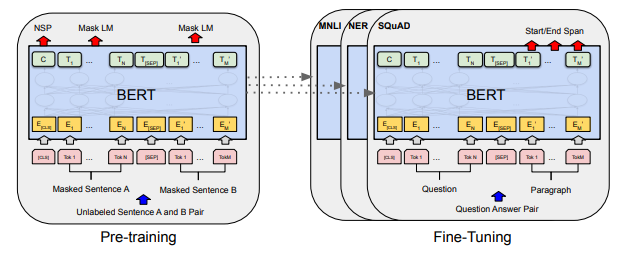
\includegraphics[width=0.7\textwidth]{styles/diploma/inc/bert1.png} 
    \caption{Общая схема предварительного обучения и дообучения модели BERT

}
    \label{fig:example}
\end{figure}


Для любого токена его входное представление формируется путём суммирования трёх компонентов:
\begin{enumerate}[label=\arabic*.]
\item эмбединга токена,

\item эмбединга сегмента (указывающего, к какому предложению он относится),
\item позиционного эмбединга.
\end{enumerate}


Визуализация этого процесса представлена на рисунке 3.

   \begin{figure}[h!]
    \centering
    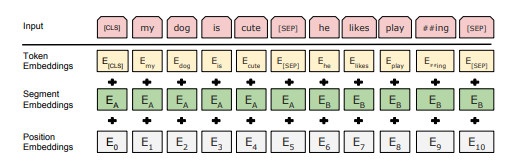
\includegraphics[width=0.7\textwidth]{styles/diploma/inc/bert2.png} 
    \caption{Представление входных данных в BERT}
    \label{fig:example}
\end{figure}

BERT не использует традиционные языковые модели, обучаемые слева направо или справа налево, для предварительного обучения BERT. Вместо этого модель обучается  на основе двух задач без учителя, описанных в этом разделе. Этот этап изображён в левой части рисунка 2

нтуитивно понятно, что глубокая двунаправленная модель потенциально более мощная, чем слева-направо модель или неглубокая конкатенация двух однонаправленных моделей. Однако стандартные условные языковые модели могут обучаться только в одном направлении, поскольку двунаправленная модель позволила бы каждому слову "видеть само себя", что делало бы предсказание тривиальным.

Чтобы обучить действительно двунаправленное представление, случайный процент токенов  маскируется во входной последовательности, и модель обучаеется  предсказывать эти токены. Эта  процедура называется  Masked Language Model (MLM) (в литературе также известна как Cloze-задача). Векторы, соответствующие маскированным токенам, подаются на выходной слой softmax поверх словаря, аналогично стандартной языковой модели.

Во всех наших экспериментах  случайным образом маскируются 15\% токенов WordPiece в каждой последовательности.

В отличие от автокодировщиков с устранением шума, здесь  предсказываются только замаскированные токены, а не восстанавливается вся последовательность.

Проблема в том, что токен [MASK] не встречается во время дообучения, что создаёт рассогласование между этапами обучения и применения. Чтобы сгладить это расхождение, выбранные токены  не всегда заменяются на [MASK]. Генератор обучающих данных действует следующим образом:

\begin{enumerate}[label=\arabic*.]
\item выбирается 15\% позиций токенов для предсказания;

\item если выбран $i-й$ токен, он заменяется:
\begin{enumerate}[label=\arabic*.]
\item на [MASK] — в 80\% случаев;
\item на случайный токен — в 10\% случаев;
\item остаётся неизменным — в 10\% случаев.
\end{enumerate}

\end{enumerate}
Затем соответствующий скрытый вектор $T_i$ используется для предсказания исходного токена с использованием функции потерь кросс-энтропии.

Многие прикладные задачи, такие как вопросно-ответные системы (QA) и логический вывод (NLI), требуют понимания связей между двумя предложениями, чего не обеспечивает языковое моделирование.

Для этого мы обучаем модель на бинарной задаче предсказания следующего предложения (NSP), которую легко сгенерировать из любого одноязычного корпуса.

Для каждой обучающей пары предложений A и B:в 50\% случаев B действительно следует за A (метка IsNext),в 50\% случаев B — это случайное предложение из корпуса (метка NotNext).

Как показано на рисунке 2, для задачи NSP используется вектор [CLS], обозначаемый как C.

Несмотря на простоту, в разделе 5.1 показано, что предобучение на этой задаче существенно улучшает производительность как в QA, так и в NLI.

 BERT передаёт все параметры модели для инициализации downstream-задач.

Данные для предварительного обучения


Процедура предварительного обучения в целом соответствует предыдущим исследованиям по языковым моделям. Мы используем два корпуса:
\begin{enumerate}[label=\arabic*.]
\item BooksCorpus (~800 млн слов),

\item англоязычная Википедия (~2.5 млрд слов).
\end{enumerate}
Из Википедии извлекаются только текстовые блоки — списки, таблицы и заголовки игнорируются.

\subsubsection{Дообучение BERT(Fine-tuning)}


Дообучение BERT выполняется просто, так как механизм самовнимания (self-attention) в трансформере позволяет использовать модель для многих задач, включая как отдельные тексты, так и пары текстов, просто заменяя входы и выходы.

Обычно в задачах с парами текстов применяют двухэтапный подход: сначала кодируют предложения по отдельности, а затем применяют перекрёстное внимание (cross-attention), как в работах Parikh и др. (2016), Seo и др. (2017).

BERT же объединяет эти этапы — кодирует сразу объединённую пару предложений с помощью self-attention, тем самым реализуя перекрёстное внимание автоматически.

Для каждой задачи  подключаются специфичные входы и выходы, и модели дообучивают всеми параметрами  от начала до конца.

На входе:

пара предложений A и B, аналогичная: <добавить нормальтный спиолк>
\begin{enumerate}[label=\arabic*.]
\item парафразам;
\item паре гипотеза–предпосылка в задачах логического вывода;
\item паре вопрос–текст в QA;
\item паре «текст–∅» в классификации или теггинге последовательностей.
\end{enumerate}

На выходе:
\begin{enumerate}[label=\arabic*.]
\item вектор токена используется для задач на уровне токенов (sequence tagging, QA),
\item вектор [CLS] используется для задач классификации (например, sentiment analysis, entailment).
\end{enumerate}
паре гипотеза–предпосылка в задачах логического вывода;

паре вопрос–текст в QA;

паре «текст–∅» в классификации или теггинге последовательностей.

На выходе:

вектор токена используется для задач на уровне токенов (sequence tagging, QA),вектор [CLS] используется для задач классификации (например, sentiment analysis, entailment).

Итоги предварительного обучения BERT:

\begin{enumerate}[label=\arabic*.]
\item Характеристика	Подробности
Корпус для пре-тренинга	BookCorpus ≈ 800 млн слов + англ. Wikipedia ≈ 2,5 млрд слов (в сумме ≈ 3,3 млрд).
\item Модели	BERT-BASE (12 блоков, 768 скрытых, 12 голов, 110 M парам.).
\item BERT-LARGE (24 блока, 1024 скрытых, 16 голов, 340 M парам.) 
arXiv.
\item Задачи пре-тренинга	1. Masked LM (MLM) — случайно маскируются 15 \% токенов и предсказываются.
\itemКлючевые результаты	Новый SOTA на 11 NLP-бенчмарках: GLUE 80,5 (+7,7 pp), MultiNLI 86,7 (+4,6 pp), SQuAD v1.1 F1 93,2 (+1,5 pp) и др. 
arXiv.
\end{enumerate}

Результаты оригинального BERT впечатляют, но из-за английского корпуса они напрямую не переносятся на русский. Для качественной работы стоит сразу брать модель, предобученную на русском и, при необходимости, дообучать её на собственной задаче.

  % Теория
\subsection{SBERT}

Кроме обучения на русских данных, SBERT также имеет ряд отличительх особенной.

Sentence-BERT (SBERT) добавляет к выходу моделей BERT операцию пулинга, чтобы получить фиксированное векторное представление предложения. Cуществует три стратегии пулинга:

\begin{enumerate}[label=\arabic*.]
\item использование выхода токена [CLS];
\item вычисление среднего по всем выходным векторам (MEAN-strategy);
\item вычисление поэлементного максимума за всё время (MAX-strategy).
\end{enumerate}

Стратегия по умолчанию — MEAN.

Для тонкой настройки (fine-tuning) BERT строются сиамские и триплет-сети, чтобы обновить веса модели так, чтобы полученные эмбединги предложений были семантически осмысленными и их можно было сравнивать по косинусному сходству.

Конкретная архитектура сети зависит от имеющихся обучающих данных. В  модели используются   следующими структуры и целевые функции.

 \subsubsection{Функция цели для классификации}:

 Объединяются (конкатенируются) эмбединги предложений $u$ и $v$ с покомпонентной разностью $∣u−v∣$ ,и  полученный вектор умножается на обучаемую матрицу весов $W_t \in \mathbb{R}^{3n \times k}$:

 
\begin{equation}
o = \mathrm{softmax}(W_t (u, v, |u - v|)) ,
\end{equation}
где:
\begin{itemize}
    \item  $n$ — размерность эмбедингов предложений;
    \item $k$ — количество классов (меток).
\end{itemize} 

В качестве функции оптимизации используется кросс-энтропийная функция потерь (cross-entropy loss). Эта архитектура показана на рисунке 4.
\begin{figure}[h!]
    \centering
    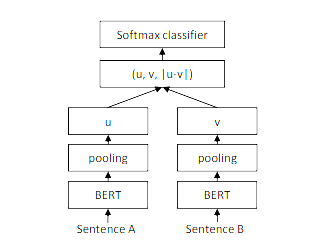
\includegraphics[width=0.7\textwidth]{styles/diploma/inc/sbert1.png} 
    \caption{Архитектура SBERT с функцией цели классификации, например, для дообучения на датасете SNLI. Две сети BERT используют общие веса (сиамская архитектура).}
    \label{fig:example}
\end{figure}


 \subsubsection{Функция цели для регрессии}. 
 
 Между двумя эмбедингами предложений}
Между двумя эмбедингами предложений $u$ и $v$ вычисляется их косинусное сходство (см. рисунок 5). В качестве целевой функции используется среднеквадратичная ошибка (mean-squared error, MSE).}


\begin{figure}[h!]
    \centering
    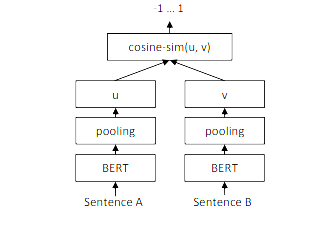
\includegraphics[width=0.7\textwidth]{styles/diploma/inc/sbert2.png} 
    \caption{Архитектура SBERT на этапе инференса, например, для вычисления коэффициентов семантического сходства между предложениями. Эта архитектура также используется с регрессионной функцией потерь.}
    \label{fig:example}
\end{figure}


  \subsubsection{Функция цели для триплетной потерь (Triplet Objective Function)}.
Имея якорное предложение 
$a$, положительное предложение $p$ и отрицательное предложение 
$n$, триплетная функция потерь настраивает сеть так, чтобы расстояние между $a$ и $p$ было меньше, чем расстояние между $a$ и $n$.

Математически, функцию потерь минимизируется следующим образом:

\begin{equation}
\max\left( \|\mathbf{s}_a - \mathbf{s}_p\| - \|\mathbf{s}_a - \mathbf{s}_n\| + \epsilon,\ 0 \right),
\end{equation}

где:
\begin{itemize}
    \item $s_x$ — эмбединги предложений $a$,$n$ или $p$;
    \item  $\|{\cdot}\|$ — метрика расстояния;
    \item  $\epsilon$ — зазор (margin).
\end{itemize}  

Значение $\epsilon$ гарантирует, что эмбединги $s_p$ находятся как минимум на $\epsilon$ ближе к $s_a$, чем $s_n$. В качестве метрики используется евклидово расстояние, и в экспериментах устанавливается $\epsilon = 1$.


 \subsubsection{Тестирование}
Результаты SBERT вместе с другими популяпными моделями, в том числе BERT.

\begin{table}[H]
\centering
\small
\caption{Скорреляции Спирмена $\rho \times 100$ для задач STS без учёта обучающих данных STS.}
\begin{tabular}{lccccccc}
\toprule
\textbf{Модель} & STS12 & STS13 & STS14 & STS15 & STS16 & STSb & SICK\textsubscript{R} & Avg.\\
\midrule
Avg. GloVe              & 55.14 & 70.66 & 59.73 & 68.25 & 63.66 & 58.02 & 53.76 & 61.32\\
Avg. BERT               & 38.78 & 57.98 & 57.98 & 63.15 & 61.06 & 46.35 & 58.40 & 54.81\\
BERT CLS                & 20.16 & 30.01 & 20.09 & 36.88 & 38.08 & 16.50 & 42.63 & 29.19\\
InferSent‐GloVe         & 52.86 & 66.75 & 62.15 & 72.77 & 66.87 & 68.03 & 65.65 & 65.01\\
USE                     & 64.49 & 67.80 & 64.61 & 76.83 & 73.18 & 74.92 & 76.69 & 71.22\\
\midrule
\textbf{SBERT-NLI-base} & 70.97 & 76.53 & 73.19 & 79.09 & 74.30 & 77.03 & 72.91 & 74.89\\
\textbf{SBERT-NLI-large}& 72.27 & 78.46 & 74.90 & 80.99 & 76.25 & 79.23 & 73.75 & 76.55\\
SRoBERTa-NLI-base       & 71.54 & 72.49 & 70.80 & 78.74 & 73.69 & 77.77 & 74.46 & 74.21\\
SRoBERTa-NLI-large      & 74.53 & 77.00 & 73.18 & 81.85 & 76.82 & 79.10 & 74.29 & 76.68\\
\bottomrule
\end{tabular}
\end{table}

\begin{table}[H]
\centering
\small
\caption{Spearman $\rho \times 100$ на тесте STSb. $\pm$ — стандартное отклонение по 10 запускам.}
\begin{tabular}{lcc}
\toprule
\textbf{Модель} &  Обучение &  $\rho$ \\
\midrule
Avg. GloVe                                  & –                      & 58.02\\
Avg. BERT                                   & –                      & 46.35\\
InferSent (GloVe)                           & –                      & 68.03\\
USE                                         & –                      & 74.92\\
\textbf{SBERT-NLI-base}                     & без STS               & 77.03\\
\textbf{SBERT-NLI-large}                    & без STS               & 79.23\\
BERT-STSb-base                              & STSb                  & $84.30\pm0.76$\\
\textbf{SBERT-STSb-base}                    & STSb                  & $84.67\pm0.19$\\
BERT-NLI-STSb-large                         & NLI+STSb              & $88.77\pm0.46$\\
\textbf{SBERT-NLI-STSb-large}               & NLI+STSb              & $86.10\pm0.13$\\
\bottomrule
\end{tabular}
\end{table}

\begin{itemize}
  \item Поиск самой похожей пары в коллекции из $10\,000$ предложений:
  \begin{itemize}
    \item \textbf{BERT} — $n(n{-}1)/2 \approx 5\times10^{7}$ сравнений $\Rightarrow$ $\sim65$ часов на V100 GPU;
    \item \textbf{SBERT} — $n$ инференсов ($\sim$5 с) + cosine-similarity ($<$0.01 с).
  \end{itemize}
  \item Тонкая настройка SBERT занимает $<20$ минут на одном GPU.
\end{itemize}


Хотя SBERT демонстрирует впечатляющие показатели качества, для конечного пользователя важна не только точность, но и время отклика системы. Чтобы снизить задержки при обработке запросов и масштабировать решение под высокую нагрузку, целесообразно развернуть модель в рамках микросервисной архитектуры: вынести SBERT-сервис в отдельный контейнер и параллелить запросы через легковесный API-шлюз. 

Таким образом возможно одновременно и сохранить высокое качество семантического поиска ,и обеспечить быстроту реакции, что критично для реальных приложений.  % Теория
\section{Микросервисы}

Микросервисы — это архитектурный подход к разработке программного обеспечения, при котором приложение состоит из небольших независимых сервисов, взаимодействующих через чётко определённые API. 

Архитектура микросервисов упрощает масштабирование приложений и ускоряет их разработку, что способствует инновациям и сокращает время вывода новых функций на рынок.


Микросервисы имеют ряд преимуществ:
\begin{enumerate}[label=\arabic*)]

   \item \textbf{Более эффективное использование ресурсов}.
Микросервисная архитектура позволяет гибко подгонять каждый сервис под конкретную нагрузку. Оптимально распределяя вычислительные ресурсы, можно добиться лучшего коэффициента их использования и грамотного масштабирования.

Например, сервису с высоким CPU-потреблением выделяют больше вычислительных ядер, тогда как сервису, которому критичен объём памяти, — больше RAM.

Такая оптимизация снижает операционные затраты приложения и повышает общую эффективность работы системы.

     \item  \textbf{Гибкое масштабирование (Flexible Scaling)}.	 Каждый сервис можно масштабировать независимо, ориентируясь на нагрузку именно той функции, которую он обеспечивает. Это позволяет точно подбирать ресурсы, понимать стоимость конкретной фичи и сохранять доступность при всплесках трафика.
   \item \textbf{Простота деплоя (Easy Deployment)	}.Микросервисы облегчают CI/CD: пробовать новые идеи и откатываться при неудаче становится дешевле. Низкая цена ошибки поощряет эксперименты и ускоряет вывод новых возможностей на рынок.
   \item \textbf{Изоляция отказов}.
Когда какой-либо сервис в микросервисной архитектуре выходит из строя, остальная система продолжает работать, поскольку каждый сервис функционирует независимо. Такая изоляция отказов повышает надёжность всей системы и облегчает разработчикам поиск и устранение неисправностей: понятно, какой именно сервис «болит».


\end{enumerate}


\begin{figure}[H]
    \centering
    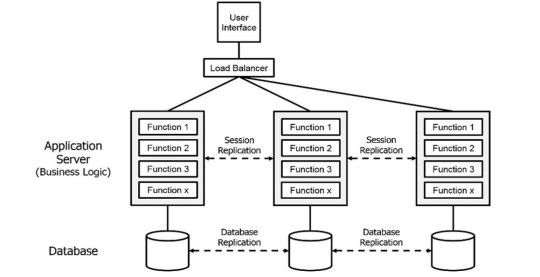
\includegraphics[width=0.7\textwidth]{styles/diploma/inc/microservice1.png} 
    \caption{Пример микросервисной архитектуры. На рисунке видно, как каждый сервис полностью независим от других сервисов.}
    \label{fig:example}
\end{figure}

Таким образом, в системе заложены ключевые принципы — изоляция отказов, гибкое масштабирование и эффективное использование ресурсов. Следующий шаг — организовать надёжное взаимодействие между микросервисами.

В выбранной архитектуре один сервис отвечает за бизнес-логику приложения, а другой — за инференс модели. Чтобы модель своевременно получала новые данные, необходим асинхронный канал обмена сообщениями. Оптимальным решением здесь становится очередь RabbitMQ



  % Теория
\section{Брокеры сообщений}
\subsection{RabbitMQ}

RabbitMQ — это программное обеспечение для организации очередей сообщений; его также называют брокером сообщений или менеджером очередей. Проще говоря, это система, в которой определяются очереди, к которым подключаются приложения, чтобы передать одно или несколько сообщений.

Сообщение может содержать любую информацию. Например, в нём могут передаваться данные о процессе или задаче, которую нужно запустить в другом приложении (возможно, находящемся на другом сервере), либо это может быть просто текстовое сообщение. Брокер хранит сообщения, пока приложение-получатель не подключится и не заберёт их из очереди. Затем получатель обрабатывает сообщение.

Брокер сообщений действует как посредник между различными сервисами (например, веб-приложением). Он позволяет снизить нагрузку и сократить время отклика веб-серверов, передавая ресурсоёмкие или длительные операции стороннему компоненту, у которого нет других задач.

Очереди сообщений позволяют веб-серверам быстро отвечать на запросы, не выполняя сразу тяжёлые вычисления, которые могли бы задержать ответ. Кроме того, очереди удобны, когда нужно доставить одно сообщение нескольким потребителям или сбалансировать нагрузку между рабочими процессами.

Потребитель забирает сообщение из очереди и начинает его обрабатывать, в то время как производитель продолжает ставить новые сообщения в очередь. Потребитель может находиться на совершенно другом сервере, чем производитель, или на том же самом. Запрос может быть сформирован на одном языке программирования, а обработан — на другом. Главное, что оба приложения взаимодействуют только через передаваемые сообщения, что обеспечивает их слабую связанность.

\begin{figure}[h!]
    \centering
    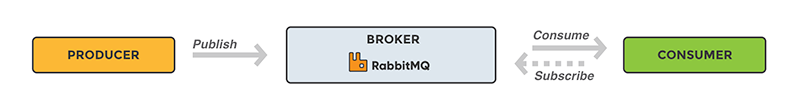
\includegraphics[width=0.7\textwidth]{styles/diploma/inc/rabbitmq1.png} 
    \caption{Общее представление работы RabbitMQ}
    \label{fig:example}
\end{figure}

Сообщения публикуются не напрямую в очередь: сначала продюсер отправляет их на exchange (обменник). Именно обменник отвечает за маршрутизацию сообщений в разные очереди с помощью биндингов и ключей маршрутизации (routing keys). Биндинг представляет собой связь между очередью и обменником.

Порядо отправки сообщения в RabbitMQ:
\begin{enumerate}[label=., leftmargin=3em]
\item Продюсер публикует сообщение в обменник. При создании обменника  обязательно указывается его тип (об этом — позже).
\item Обменник получает сообщение и решает, как его направить. При этом он учитывает тип обменника и свойства сообщения, например routing key.
\item К обменнику создаются биндинги, связывающие его с очередями. На рисунке показано два биндинга к двум различным очередям. В зависимости от атрибутов сообщения обменник маршрутизирует его в соответствующие очереди.
\item Сообщения остаются в очереди, пока их не обработает консьюмер.

\item Консьюмер извлекает сообщение из очереди и выполняет необходимую обработку.
\end{enumerate}

\begin{figure}[h!]
    \centering
    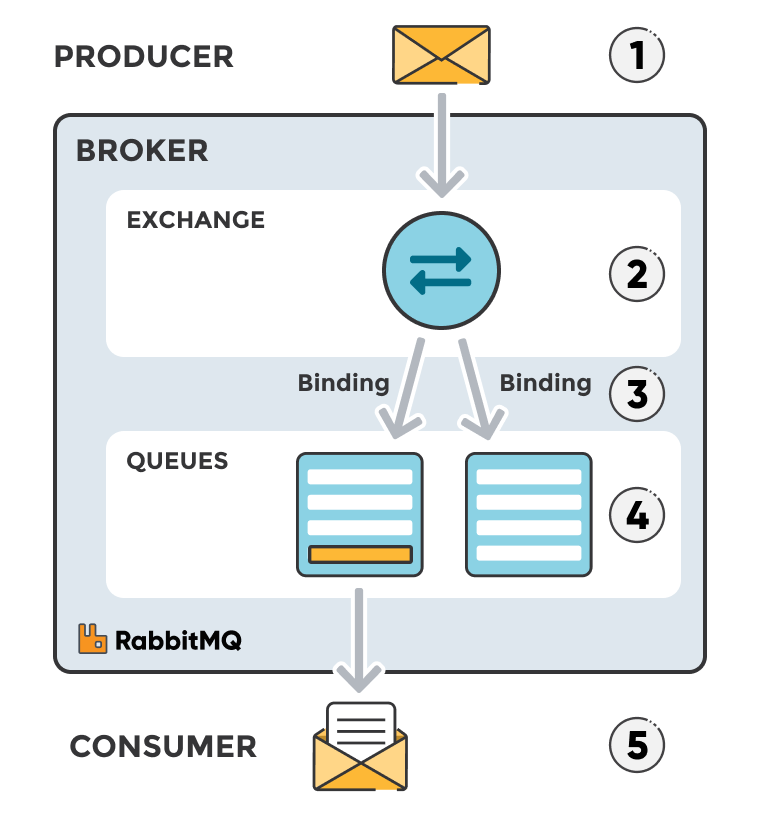
\includegraphics[width=0.5\textwidth]{styles/diploma/inc/rabbitmq2.png} 
    \caption{Устройство обменников в RabbitMQ}
    \label{fig:example}
\end{figure}







  % Теория
\section{База данных}
\subsection{PostgreSQL}

PostgreSQL— это мощная объектно-реляционная система управления базами данных (ORDBMS) с открытым исходным кодом, известная своей надёжностью, сохранностью данных и богатым набором возможностей. Она поддерживает расширенные типы данных, сложные запросы, внешние ключи, триггеры, представления, а также процедурные языки для хранения процедур. PostgreSQL легко расширяется: пользователи могут добавлять новые функции, типы данных и другие возможности. Жёсткое соблюдение стандартов SQL и поддержка свойств ACID (атомарность, согласованность, изолированность, надёжность) делают PostgreSQL идеальным выбором для разработчиков и компаний, которым нужна масштабируемая, эффективная и безопасная база данных.

Выбор PostgreSQL в качестве СУБД даёт уникальное сочетание преимуществ, отвечающих самым разным требованиям к управлению данными. Одно из ключевых достоинств — превосходная поддержка продвинутых типов данных и расширенного функционала. В их числе — нативная работа с JSON, геометрическими данными и пользовательскими типами, что обеспечивает гибкое и эффективное хранение и извлечение информации под самые сложные и разнообразные модели данных. Способность PostgreSQL легко обрабатывать сложные запросы, транзакции и масштабные операции хранилищ данных делает СУБД отличным выбором для приложений, требующих глубокой аналитики, обработки в реальном времени и высокой целостности данных.

PostgreSQL обладает множеством преимуществ, которые делают её превосходным решением для самых разных задач управления данными. СУБД известна своей надёжностью, богатым функционалом и гибкостью, позволяя эффективно решать сложные задачи обработки и управления данными. Система ориентирована на поддержку крупномасштабных приложений и хранилищ, что даёт возможность строить масштабируемые и защищённые решения.

Одной из сильных сторон PostgreSQL является исключительная гибкость и расширяемость: пользователь может адаптировать базу под свои потребности. СУБД поддерживает широкий спектр встроенных и пользовательских типов данных и предоставляет несколько процедурных языков для написания хранимых процедур. Благодаря этому можно расширять возможности системы собственными функциями, операторами и новыми языками, обеспечивая эволюцию PostgreSQL вместе с развитием проекта.

PostgreSQL также отличается высокими производительностью и масштабируемостью, легко справляясь с большими объёмами данных и множеством параллельных транзакций. СУБД применяет продвинутые методы оптимизации для эффективного хранения и извлечения информации, что делает её подходящей для высоконагруженных систем. Архитектура предусматривает горизонтальное масштабирование, партиционирование и репликацию, позволяя приложениям без труда расти вместе с увеличением объёма данных и числа пользователей.

Благодаря мощным средствам оптимизации запросов PostgreSQL эффективно выполняет сложные выборки. Среди её инструментов — index-only scans, bitmap heap scans и генетический планировщик запросов, которые сокращают время их выполнения. Всё это делает PostgreSQL идеальной для задач аналитики и бизнес-интеллекта, где требуются быстрое и точное извлечение данных.

  % Теория


\practic


\section{Архитектура}
Цель – разработать высокопроизводительный систему кластеризации документов, которая принимаем документ (PDF, DOCX), генерирует кластеры для извлеченных текстовых данных и сохраняет результат в графовом виде. 

Как было упомянуто в теоритической части, приложение реализовано с использованием микросервисной архиктеруры. Подробно расскажем о ней:

\begin{figure}[h!]
    \centering
    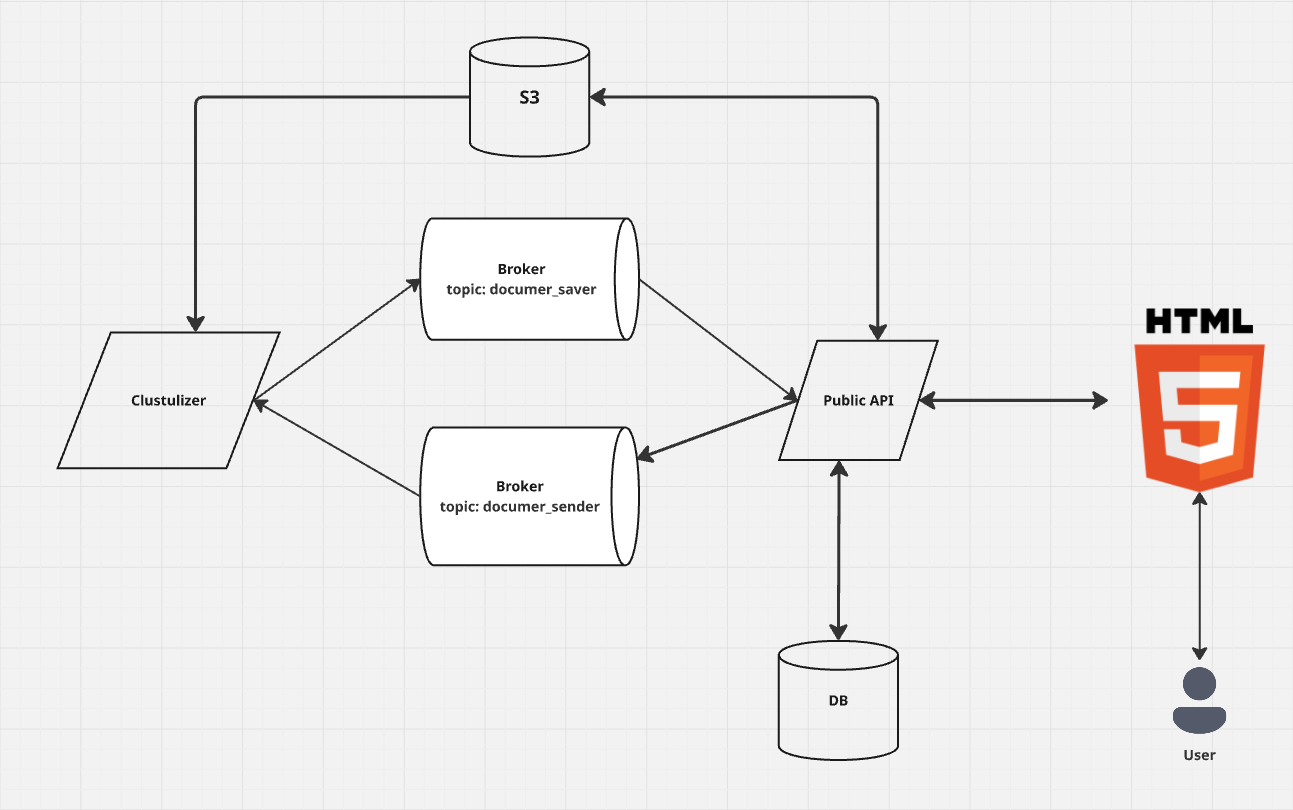
\includegraphics[width=1\textwidth]{styles/diploma/inc/microservice2.png} 
    \caption{Архитектура приложения}
    \label{fig:example}
\end{figure}
Система состоит из 5 компонентов:
\begin{itemize}
    \item S3 (Simple Storage Service);
    \item Broker;
    \item DB;
    \item  Сервис  Public AP;
    \item Сервис  Clusterizer;
    \item Пользовательский интерфейс.
    
  \end{itemize}
\subsection{Логика приложения}
\begin{enumerate}[label=\arabic*)] 
\item Пользователь загружает файл в графическом интерфейсе;
\item Пользовательский интерфейс совершает AJAX-запрос и ждет ответа сервера;

\item Сервер возвращает уникальный ID, который frontend сохраняет в виде cookie данных. Запускается периодическяа фукнция, делающая с заданным интервалом AJAX-запрос к Public API для получния статуса обработки документов;

\item Файл попадает в Public API. Добавляется запись в  DB о создании новой заявки на обработку. Файл отправляется в broker на топик processing, а также сохраняется в хранилище S3;
\item Clustulizer получает сообщения из топика processing , обрабатывает  и передает результат в топик save;
\item Public API читает топик брокера save, получает результат обработки  и сохраняет его в БД;
\item Пользователь получает результат в графическом интерфейсе.
\end{enumerate}

\section{Компоненты приложения}
Подбробнее расскажим об каджой компоненте

\subsection{S3}

В проекте хранилище S3 необоходимо для управления файлами пользователя. Система не ограничивает размер входных данных, поэтому было решино использовать данную технологию.

Как было отмечено в теоретической части, S3 — это всего лишь API, а значит, любой провайдер может реализовать совместимый способ хранения данных. В рамках архитектуры моего проекта я рассматриваю несколько поставщиков облачных хранилищ, каждый из которых предлагает S3-интерфейс с различными характеристиками.

\begin{itemize}
    \item \textbf{Yandex Cloud:}'
    
    Российская облачная платформа с развитой экосистемой сервисов, включая облачное хранилище с полной поддержкой S3 API. Отличается стабильной производительностью, хорошей документацией и активной технической поддержкой. Локализована, соответствует российским требованиям по хранению данных и регулярно обновляется. Yandex Object Storage легко интегрируется с микросервисной архитектурой и поддерживает IAM, версионирование, классы хранения и шифрование на стороне сервера.
    \item \textbf{СберCloud:}
    
    Платформа от Сбера, ориентированная на корпоративный сектор и государственные организации. Также предоставляет S3-совместимое хранилище, но часто предполагает более сложную бюрократическую процедуру подключения и настройки. Имеет сильную интеграцию с инфраструктурой Сбера, но менее гибка и медленнее обновляется по сравнению с конкурентами.
    \item \textbf{VK Cloud:}
    
    Ещё один крупный российский провайдер с поддержкой S3. VK Cloud предлагает интересные тарифы и технически надёжную реализацию. Однако экосистема менее развита, чем у Яндекса, а документация и поддержка не всегда оперативны.
   
  \end{itemize}

  Хотя каждый из представленных провайдеров предлагает базовую поддержку S3-интерфейса, Yandex Cloud наиболее полно сочетает в себе техническую зрелость, простоту интеграции, гибкие тарифы и совместимость с современными DevOps-инструментами. В контексте микросервисной архитектуры с ML-компонентами, где важны скорость, стабильность и автоматизация, выбор очевиден — Yandex Object Storage.

\subsection{Broker}

Broker является очередью сообщений. В роли очереди используется RabbitMQ.
Данная компонента система необходимо для передача данных от одного сервиса к другому. 

Приложение должно удолетворять критериям скорости и наджености. В системе Broker решает сразу оба:
\begin{itemize}
    \item \textbf{Надежность}. Если некоторый запрос зависнит,потеряет и т.п, то он сохранится в памяти брокера, поэтому  клиенты получать результат практически в 100\% случаев
     \item \textbf{Скорость}. Брокер способен балансировать пришедшие на него сообщения, то есть он будет выбирать только доступные репликации другого микросервиса, что особенно важно для пользовательского опыта.
\end{itemize}
\subsection{DB}

DB представляет собой объектно-реляционную базу данных. Благодаря выбранной архитектуре   микросервисов( о которой погорим далее), можно выбрать любую базу данных.

Я остановился на PostgresQL. Кратко пройдусь по причинам ее выбора:
\begin{itemize}
\item  \textbf{Поддержка сложных запросы, транзакции и индексацию}. Любая система, подразумевающая себя высоконагруженной, обязательно должно иметь следущих список технологий.Особеноно важным является индекс.

Индексы в PostgreSQL — это важный механизм оптимизации, который позволяет ускорить выполнение запросов за счёт сокращения количества просматриваемых строк в таблице. Вместо полного прохода по таблице (что может занимать значительное время при большом объёме данных), индекс позволяет базе быстро определить, где находятся нужные записи. PostgreSQL поддерживает разнообразные типы индексов (B-tree, Hash, GIN, GiST и другие)
\item \textbf{Поддержка JSON}. Позволяет удобно хранить и обрабатывать как структурированные, так и полуструктурированные данные в одной базе. 
\end{itemize}

База данных содержит 2 таблицы  - request и file.
\begin{table}[H]
\centering
\caption{Структура таблицы \texttt{request}}
\begin{tabular}{|l|l|l|}
\hline
\textbf{Поле} & \textbf{Тип данных} & \textbf{Описание} \\
\hline
\texttt{id}          & UUID            & Первичный ключ \\
\texttt{result}      & JSONB           & Результат запроса (в JSON) \\
\texttt{status}      & varchar(50)     & Статус запроса \\
\texttt{created\_at} & TIMESTAMP       & Дата создания (по умолчанию \texttt{now()}) \\
\texttt{updated\_at} & TIMESTAMP       & Дата обновления (по умолчанию \texttt{now()}) \\
\hline
\end{tabular}
\end{table}

Таблица request необходима для учета пользователей запросов  обработки документов. Подробно расскажу о каждом поле:
\begin{itemize}
\item  \textbf{id}. Уникальный индификатор. Необходим для корректной работы пользовательского интверфейса;
\item  \textbf{result}. Содержит результат обработки документов кластеризатором;
\item \textbf{status}. Показывает состояние запроса в данный момент;
\item \textbf{created\_at}, \textbf{updated\_at}. Метаданные, необходимые для аналитики и отслеживания работы системы. 

Поле \textbf{created\_at} фиксирует момент создания записи, а \textbf{updated\_at} — время последнего изменения. Эти данные позволяют анализировать активность, выявлять задержки и отслеживать возможные проблемы в системе.
\end{table}


\begin{table}[H]
\centering
\caption{Структура таблицы \texttt{file}}
\begin{tabular}{|l|l|l|}
\hline
\textbf{Поле} & \textbf{Тип данных} & \textbf{Описание} \\
\hline
\texttt{id}   & UUID          & Первичный ключ \\
\texttt{type} & varchar(30)   & Тип файла \\
\texttt{key}  & varchar(100)  & Ключ \\
\texttt{title}& varchar(255)  & Название \\
\hline
\end{tabular}
\end{table}

Таблица file необходима для учета файлов для даленьшего удобного скачивания нужного файла. Подробно расскажу о каждом поле:
\begin{itemize}
\item  \textbf{id}. Уникальный индификатор. Необходим для корректной работы пользовательского интверфейса;
\item  \textbf{type}. Содержит формат файла(docx или pdf);
\item \textbf{status}. Показывает состояние запроса в данный момент;
\item \textbf{key}. Индификатор файла, по которому он сохранен в S3
\item \textbf{title}. Полученное название файла

Поле \textbf{created\_at} фиксирует момент создания записи, а \textbf{updated\_at} — время последнего изменения. Эти данные позволяют анализировать активность, выявлять задержки и отслеживать возможные проблемы в системе.
\end{itemize}

\subsection{Сервис Public AP}
Public API является легковесным HTTP-сервером. Данный компонент является своего рода входного узла.  Он не влючает в себя тяжелую CPU Bound нагрузку, а лишь I/O Bound. 
Все поользовательские запросы обращаются именно к нему, а Public API общается с другими сервисами.

Public API использует следующие технологии:
\begin{itemize}
\item  \textbf{Golang}. Компилируемый язык, обеспечивающий высокую скорость чтения/записи. Облагает встроенными структурами данных (такими как горутины и каналы), которые позволяют эффективно управлять параллелизмом и конкуренцией, что особенно важно для микросервисных архитектур

Для конкретнно данного микросервиса можно было выбрать любой другой язык, но философия Golang изначально подразумевает микросервисную архитектуру, поэтому эта технология более подхоядщяая, нежели другие.
\item  \textbf{Fiber}. Cовременный высокопроизводительный легковесный веб-фреймворк для Golang. Разработан для создания микросервисов;
\item \textbf{pgxv5}. драйвер-библиотека с  взаимодействия с PostgreSQL для языка Golang.

\end{itemize}

Public API написан с использованием луковой архитектуры - паттерна, который направлен на улучшение гибкости, тестируемости и устойчивости приложения к изменениям. Он помогает отделить бизнес-логику от инфраструктурных деталей, минимизируя связность между компонентами системы.

\begin{figure}[H]
    \centering
    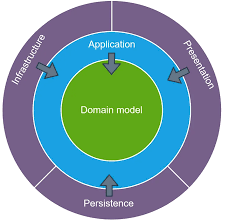
\includegraphics[width=0.5\textwidth]{styles/diploma/inc/onion1.png} 
    \caption{Устройство луковой  архитектуры}
    \label{fig:example}
\end{figure}

Микросервис состоит из 3-х слоев:
\begin{itemize}
\item  \textbf{Storage}
\item  \textbf{Service}
\item  \textbf{Handler}
\end{itemize}
Подробно расскажем о каждом из них

\subsubsection{Storage}
Отвечает за взаимодействие с базой данных.
Все методы имеют примерно одинаковую структуру:
\begin{itemize}
\item Аргумент params содержит данные, необходимые для совершения запроса к БД. Это могут быть как данные для изменения, так фильтры для возвращения данных.
\item  Запрос к базе данных через ранее инициализированный клиент PostgreSQL (метод client.Query).
Клиент представляет собой преднаписанную структуру, позволяющую совершать транзакционные запросы, что череезвычно важно в подобных проектах.
\item  Получение и преобразование данных (pgx.CollectOneRow или pgx.CollectRow и requestToEntity соответсвенно )
\end{itemize}



\begin{figure}[H]
    \centering
    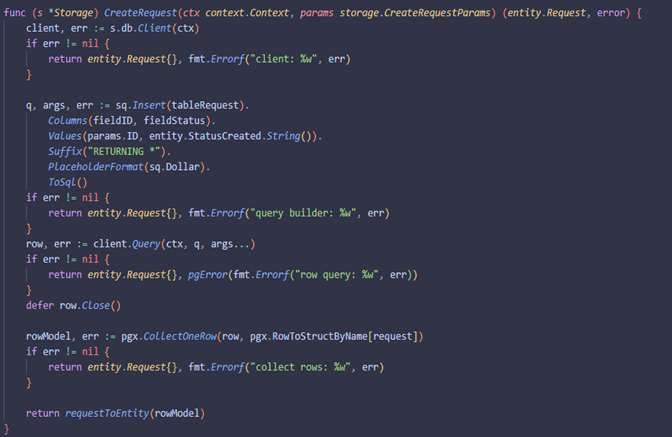
\includegraphics[width=1\textwidth]{styles/diploma/inc/storage1.png} 
    \caption{Пример метода слоя Storage -  функция создания пользовательского запроса.}
    \label{fig:example}
\end{figure}

\subsubsection{Service}

Содержит основную бизнес-логику приложения.

Бизнес логикой может являться как полноценный алгоритм(например,как на рисунке 12. В дополнению к предыдуему пункту видно использование тракзакций), так и обертка вокруг другого слоя для поддержания слоистой архитектуры.

Service использует методы слоя Storage. Важно отметить, что Service получает интерфейс Storage, то есть он не знает какая реализация лежит за этим интерфейсом. Это позволяет пластично менять технологии проекта, не затрагивая основную бизнес логику.



\begin{figure}[H]
    \centering
    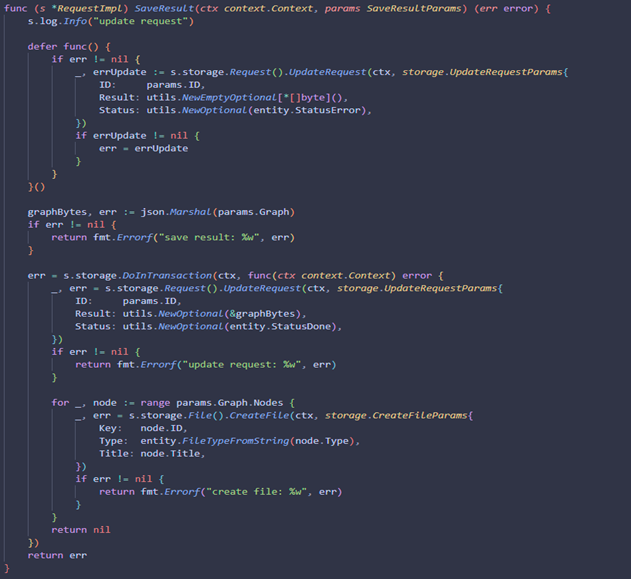
\includegraphics[width=1\textwidth]{styles/diploma/inc/service1.png} 
    \caption{Метод SaveResult}
    \label{fig:example}
\end{figure}

\begin{figure}[H]
    \centering
    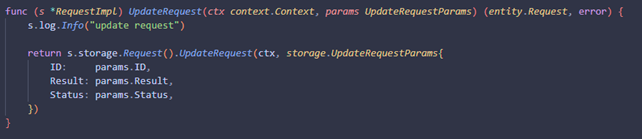
\includegraphics[width=1\textwidth]{styles/diploma/inc/service2.png} 
    \caption{Метод UpdateRequest}
    \label{fig:example}
\end{figure}

\subsubsection{Handler}
Handler - dходная точка для обработки пользовательских запросов. Чащего всего она предславляет собой методы, вызывающиеся при сетевом запросе.
В моем случае - это HTTP запросы.

В слое Handler происходит “склейка” ранее написанных  методов в слое Service. На рисунке 14 представлен метод загрузки пользовательских файлов. Стоит рассказать о каждой шаге в этом методе:

\begin{enumerate}[label=\arabic*.]
\item Строки 46-48, структура \textbf{uploadFilesRequest}  – требуемый вид запроса для метода;
\item Строки 50-52, структура \textbf{uploadFilesResponse}  – требуемый вид ответа для метода;
\item Строки 57-62, метод \textbf{h.getUploadFilesFromForm}  – обработка входных данных в понятном для языка виде;
\item Строки 64-72, метод \textbf{h.requestSrvc.CreateRequest }  – создание в БД записи нового пользовательского запроса;
\item  Строки 73-85, метод \textbf{h.s3Srvc.Upload}  - Создание уникальных индификаторов для файлов и их сохранение в хранилище S3  с помощью метода h.s3Srvc.Upload; 
\item  Строки 86-94, метод \textbf{h.documentSrvc.SendDocumentNames}  - отравка уникальных ключей файлов для дальнешней обработки на брокер сообщений.
\end{enumerate}

\begin{figure}[H]
    \centering
    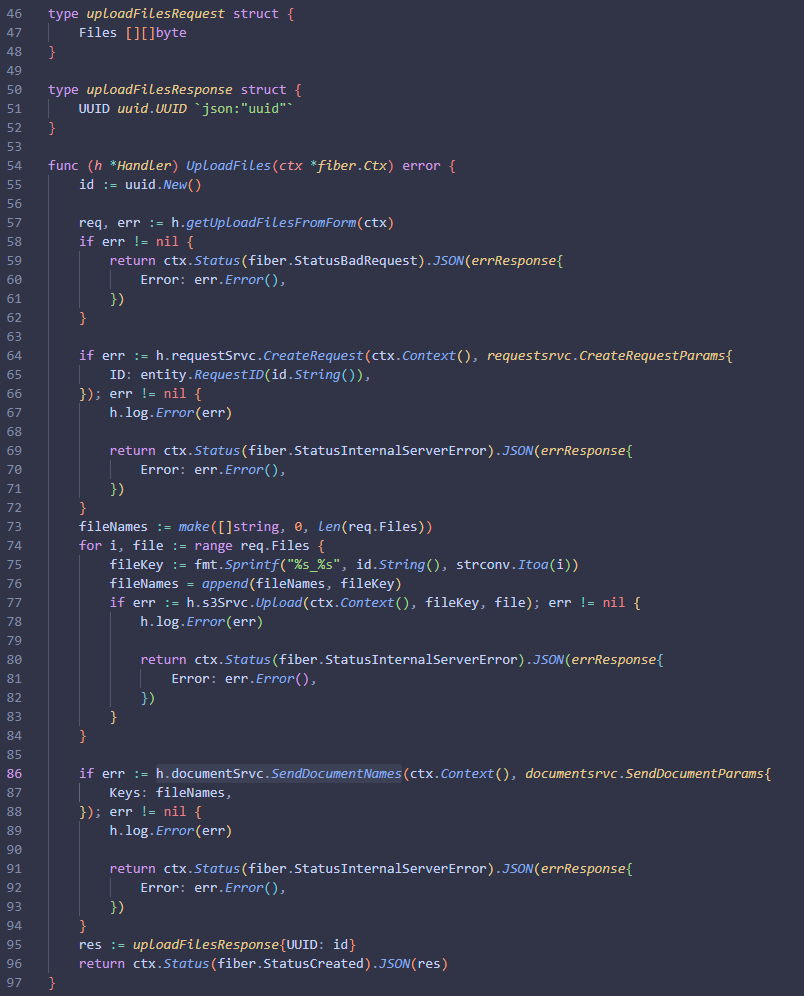
\includegraphics[width=1\textwidth]{styles/diploma/inc/handler1.png} 
    \caption{Метод UploadFiles для загрузки пользовательских файлов}
    \label{fig:example}
\end{figure}

\subsection{Сервис Clustulizer}
Clustulizer -  модуль кластеризации документов, который принимаем документ (PDF, DOCX), генерирует кластеры для извлеченных текстовых данных и возвразает результат в графовом виде

Clustulizer использует следующие технологии:
\begin{itemize}
\item  \textbf{Python} - нтерпретируемый язык,широко используется в задачах анализа данных и машинного обучения. Мой выбор пал на него в виду того, что большиство библиотек для анализа данных и кластеризации написаны именно на нем.


\item  \textbf{Sentense Tranformers }.– высокоуровневая библиотека для python, на основе transformers, предназначена для генерации эмбеддингов слов, предложений и целых документов для последующего семантического поиска похожих, может работать с большим количеством моделей, в данной работе выбрана SBERT-LARGE-NLU-RU.
\item \textbf{Модель SBERT-LARGE-NLU-RU}– модель, которая наиболее эффективна среди других моделей, обученных на русских текстах.
\item \textbf{FastAPI }– современный высокопроизводительный асинхронный веб-фреймворк для python. Его выбор обусловлен его быстротой, асинхронностью, строгой типизаци (он использует pydantic), быстротой написания кода, а также автоматической генерации документации swagger, вместе с ним используется uvicorn – легковесный, высокопроизводительный ASGI-сервер.
\end{itemize}

Clustulizer использует такую же слоистую архитектуру, как Public API.
Рассмотрим каждый слой.
\subsubsection{Storage}
Clusterlizer не взаимодействует с БД, поэтому этот слой пустой. Связано это с тем, что микросервисная архитектура требуют, чтобы у каждого сервиса была своя база данных, иначе может возникнуть сильная связанность, и смысл самой архитектуры потеряется. Все записи в базу данных выполняет сервис Public API.
\subsubsection{Service}

 Слой Service состоит из 3 классов: Converter, S3, ClusterGraphBuilder, но отдельное внимание обратим лишь на ClusterGraphBuilder, так как первые 2 по сути являются обертками вокруг python-библиотек.

Бизнес-логика ClusterGraphBuilder состоит из 3 частей:

 \begin{itemize}
\item  \textbf{Предобработка текста:}

На этом этапе подготавливается сырой текст к подаче в модель для эмбединга. Такая предобработка критически важна: она помогает устранить "шум" и выделить чистое, нормализованное представление смысла.

Алгоритм представлен на рисунке 15
\begin{figure}[H]
    \centering
    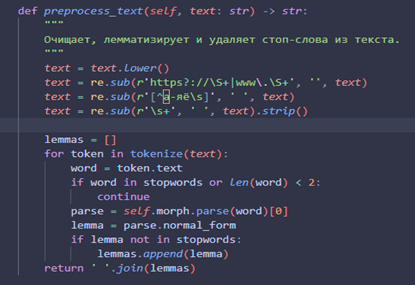
\includegraphics[width=1\textwidth]{styles/diploma/inc/clustulizer1.png} 
    \caption{Предобработка сырого документа}
    \label{fig:example}
\end{figure}

\item  \textbf{Кластеризация:}

 Это центральная часть всего сервиса  ClusterGraphBuilder, в которой «сырые» векторные представления преобразуются в осмысленные кластеры.

На рисунке 16 можно увидеть как:

 \begin{enumerate}[label=\arabic*)] % (1) (2) (3)

 \item  каждый переданный текст в метод предобрабатывается(строка 125);
\item  rаждому тексту сопоставляется его векторное представление с помощью модели  SBERT\_LARGE\_NLU\_RU(строка 129.

 Это переводит тексты из словесного пространства в числовое векторное пространство, благодаря чему можно применять методы машинного обучения;

\item применяется алгоритм HDBSCAN — продвинутый метод плотностной кластеризации, который на основании эмбедингов определяет кластеры и возвращает лейблы кластеров для каждого текста(строки 131-132);
\item пенерируются названия для файлов(строка titles).

\end{enumerate}

\begin{figure}[H]
    \centering
    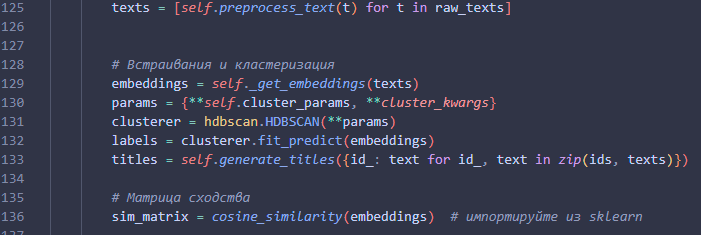
\includegraphics[width=1\textwidth]{styles/diploma/inc/clustulizer2.png} 
    \caption{Кластеризация}
    \label{fig:example}
\end{figure}


\item  \textbf{Представление в виде графа:}

На рисунке 17 представлен код преобразования входных документов в графы.

\begin{figure}[H]
    \centering
    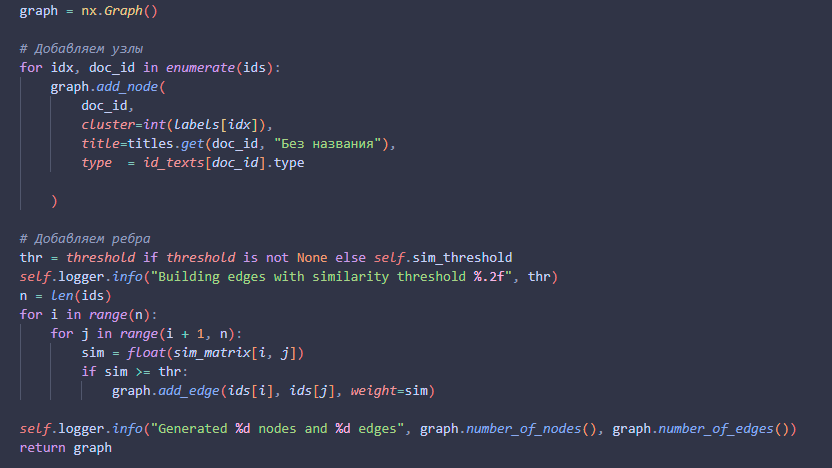
\includegraphics[width=1\textwidth]{styles/diploma/inc/clustulizer3.png} 
    \caption{Кластеризация}
    \label{fig:example}
\end{figure}
\end{itemize}

\clearpage Метод возвращает граф в виде JSON, который имеет вид:

\begin{Verbatim}[fontsize=\small]
{
  "directed": false,
  "multigraph": false,
  "graph": {},
  "nodes": [
    { "id": "Методология ML", "label": "Методология ML" },
    { "id": "Методы ML", "label": "Методы ML" },
    { "id": "Платная рыбалка", "label": "Платная рыбалка" },
    { "id": "Рыбалка Хобби", "label": "Рыбалка Хобби" }
  ],
  "links": [
    { "weight": 0.8477962017, 
    "source": "Методология ML", "target": "Методы ML" },
    { "weight": 0.959409, 
    "source": "Методология ML", "target": "Платная рыбалка" },
    { "weight": 0.768083, 
    "source": "Методология ML", "target": "Рыбалка Хобби" },
    { "weight": 0.784382, 
    "source": "Методы ML", "target": "Платная рыбалка" },
    { "weight": 0.793544,
    "source": "Платная рыбалка", "target": "Рыбалка Хобби" }
  ]
},
\end{Verbatim}
где:
  \begin{itemize}
        \item weight - весь связи, характеризующий, насколько близки 2 вершины;
        \item source, target —  грани, между которыми подсчитан вес.
    \end{itemize}
  

\subsubsection{Handler}
Слой состоит из одного класса  -  RabbitMQServer. Рассмотрит основной метод - обработку входящего сообщения:
 \begin{itemize}
 \item  Микросервис получает сообщение (строчки 61-62);
 \item  Загружает файлы из S3 хранилища (строчка 65);
 \item  Кластеризирует документы  (строчка 69);
 \item  Отправляет результат брокер сообщений   (строчки 73-75).

\end{itemize}

\begin{figure}[H]
    \centering
    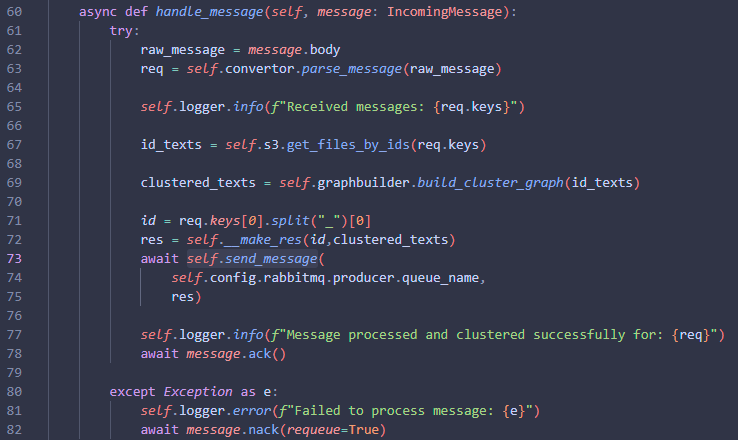
\includegraphics[width=1\textwidth]{styles/diploma/inc/clustulizer_handler1.png} 
    \caption{Метод обработки входящего сообщения на микросервис Clustulizer}
    \label{fig:example}
\end{figure}

\subsubsection{Оценка качества кластеризации и производительности}

Качество кластеризации оценивалось с использованием следующих метрик:

\begin{itemize}
    \item \textbf{Silhouette Score} — показывает, насколько объект внутри кластера схож с другими объектами этого же кластера и отличается от объектов других кластеров. Значение варьируется от $-1$ (плохая кластеризация) до $1$ (идеальная кластеризация), где значения, близкие к $0$, означают наложение кластеров.

    Формула Silhouette Score:
    \begin{equation}
    S = \frac{b - a}{\max(b, a)}  
    \end{equation}
    где:
    \begin{itemize}
        \item $a$ — среднее расстояние до объектов своего кластера;
        \item $b$ — среднее расстояние до объектов ближайшего соседнего кластера.
    \end{itemize}

    \item \textbf{Индекс Дэвиса-Болдина (Davies-Bouldin Index)} — учитывает среднее расстояние между кластерами и их радиусы. Меньшие значения указывают на более чёткие и разделённые кластеры.

    Формула DB Index:
    \begin{equation}
    DB = \frac{1}{n} \sum_{i=1}^{n} \max_{j \ne i} \left( \frac{d_i + d_j}{d_{ij}} \right)
    \end{equation}
    где:
    \begin{itemize}
        \item $d_i$ — среднее расстояние между объектами внутри $i$-го кластера,
        \item $d_{ij}$ — расстояние между центроидами кластеров $i$ и $j$.
    \end{itemize}
\end{itemize}
Тесты проводились на сгенерированных данных с моделированием через KMeans, чтобы колиество лейблов было строго заданным. 
По результатам тестов система показала высокий Silhouette Score и низкий Davies-Bouldin Index: $0.923$ и $0.107$ соответственно, что указывает на эффективность кластеризации большинства документов, тем не менее результаты могут отличаться от реальных данных.

\begin{figure}[H]
    \centering
    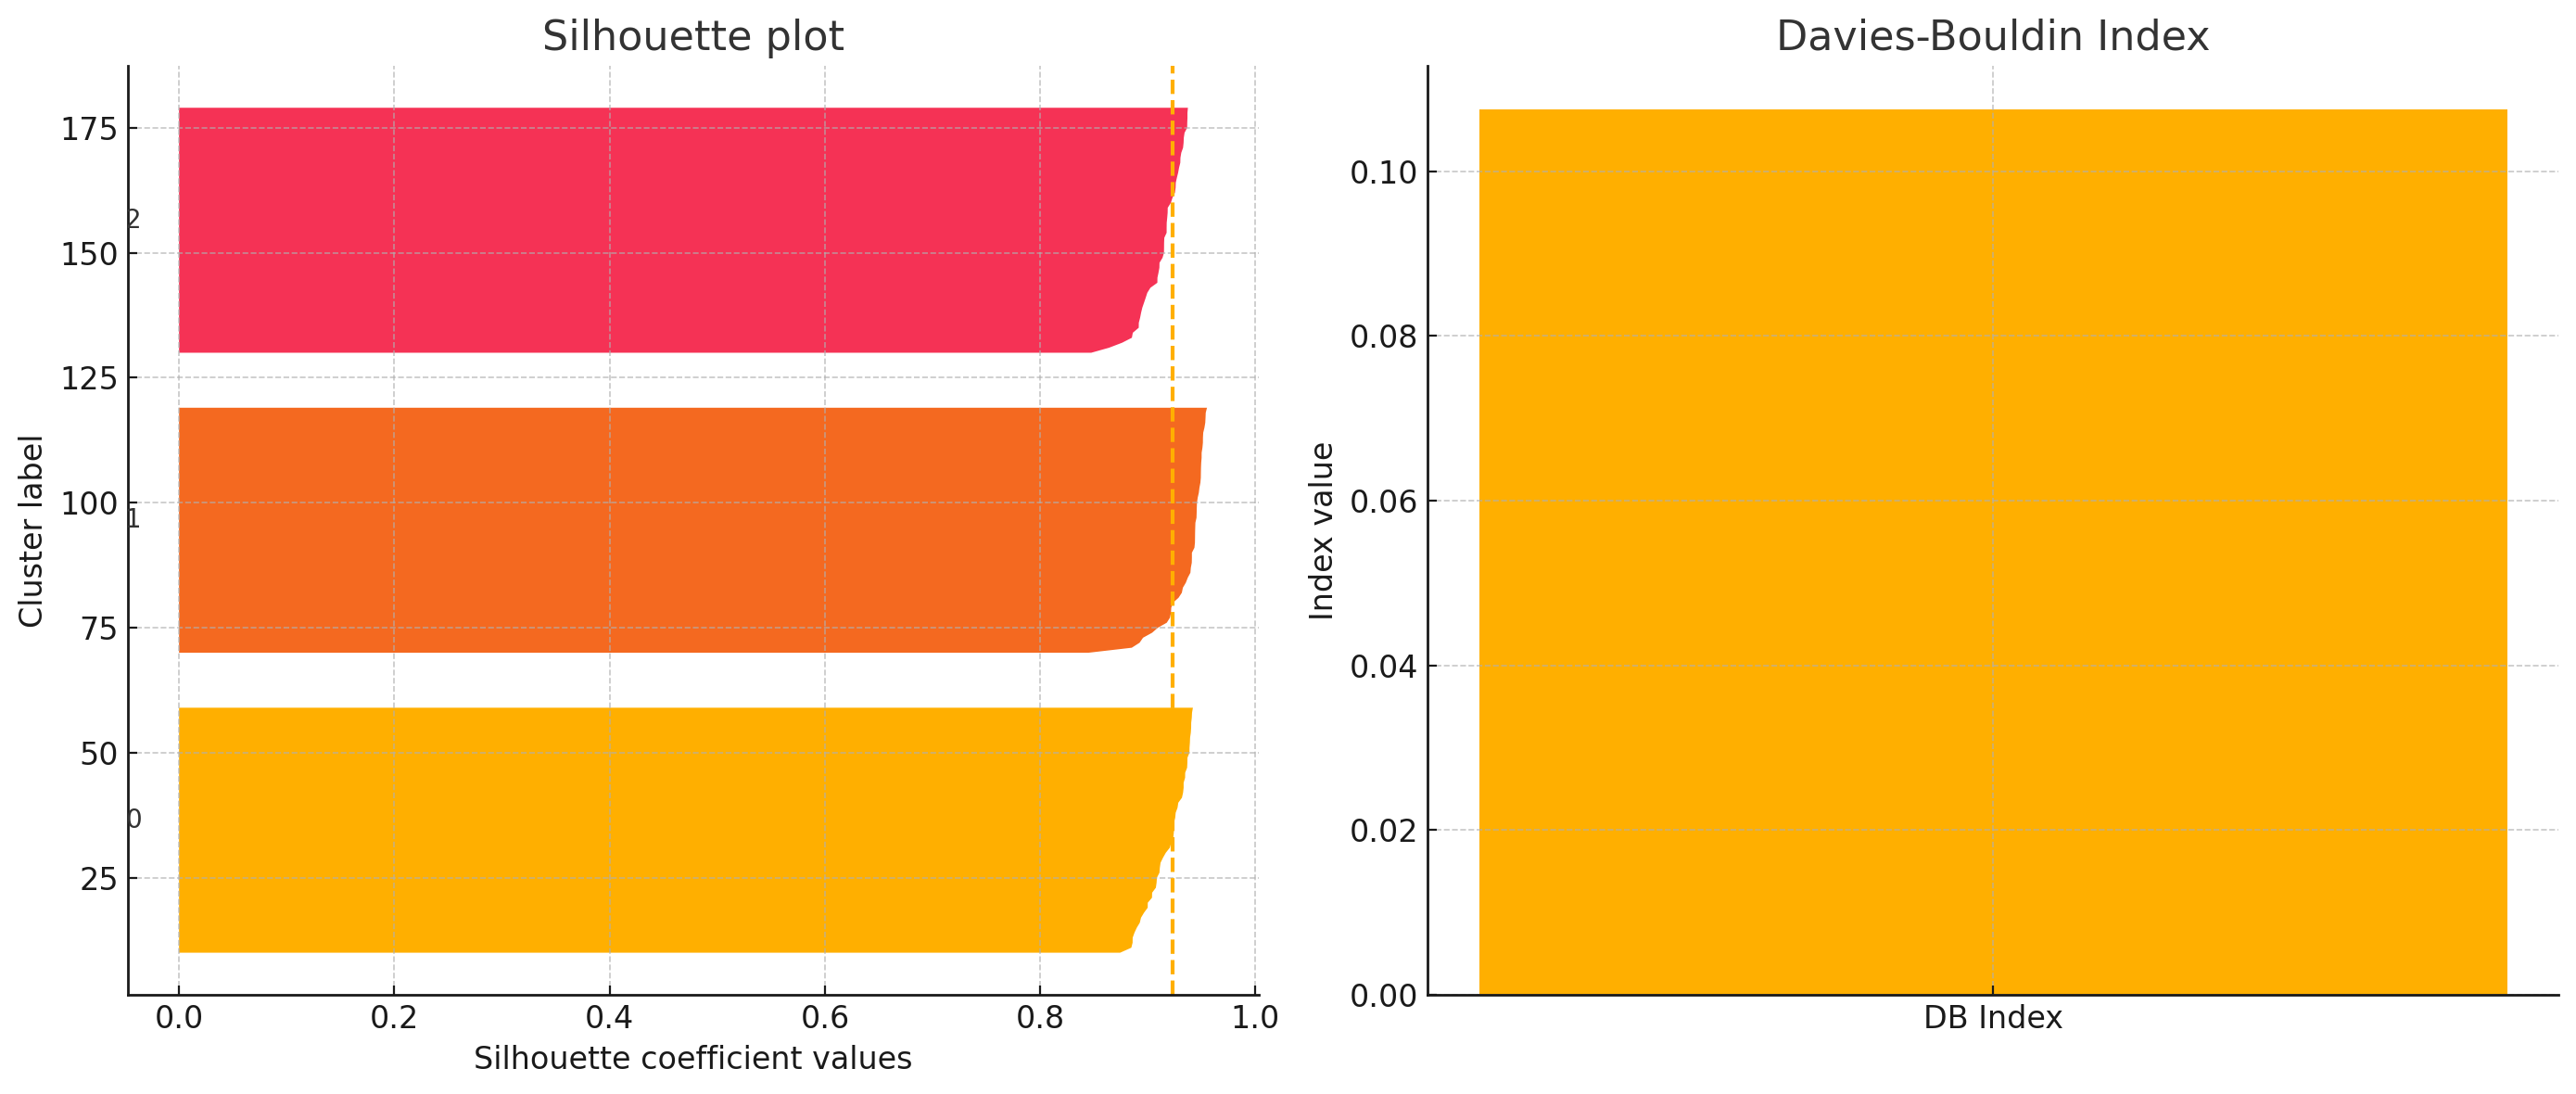
\includegraphics[width=1\textwidth]{styles/diploma/inc/clusturizer_tests1.png} 
    \caption{Результаты тестирования кластеризатора}
    \label{fig:example}
\end{figure}

\vspace{1em}

\textbf{Оценка производительности} проводилась по следующим параметрам: время ответа, пропускная способность, нагрузка на процессор и память. Полученные результаты:
\begin{itemize}
    \item Среднее время ответа — 120 мс;
    \item Загрузка процессора — 60\%;
    \item Пропускная способность — 40 документов в секунду;
    \item Использование памяти — 6 ГБ.
\end{itemize}

\subsection{Пользовательский интерфейс}
Пользовательский интерфейс представляент собой удобную обертку Public API. Для целостного использования сервиса достаточно открытого API, но для пользователя это может доставлять неудобство.
К тому же, интерфейс предсталвяет результат в виде графа, который наглядно показывает, как обработанные документы относятся  к друг другу.

Интерфейс использует ванильный JavaScript, CSS и HTML. Хоть и оформление выглядит минималистично, и если бы использовались другие технологии(например, как ReactJS и HTMX) , оболочка могла смотреться более современно. Однако благодаря этому скорость работы показывает отличные показатели. В будущем приложение обязательно  обзаводется более интересным дизайном с сохранением текущей скорости работы.


\begin{figure}[H]
    \centering
    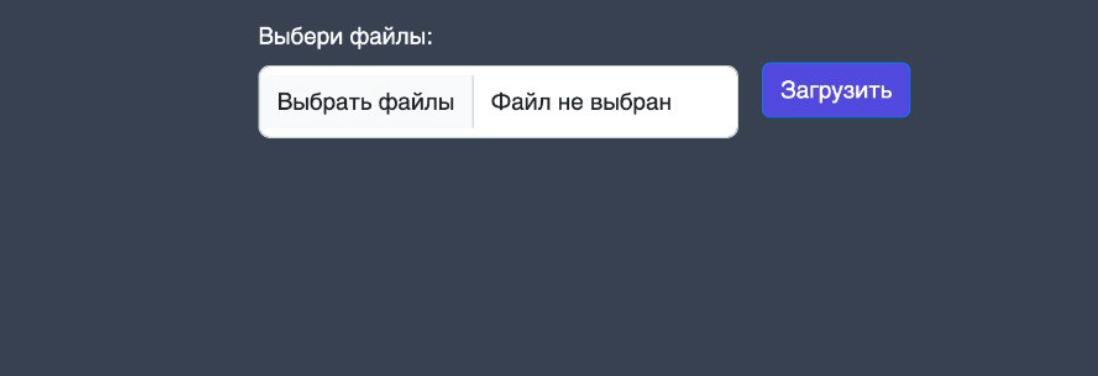
\includegraphics[width=1\textwidth]{styles/diploma/inc/front2.png} 
    \caption{Меню загрузки файлов}
    \label{fig:example}
\end{figure}


На рисунке 21 виден результат обработки, введенных пользователем документов. Цветом обозначается кластер. На рисунке 21 2 цвета : синий и желтный. Ребра между вершинами графка показывает, насколько эти вершины близки. Настраивается с помощью матрицы смежности и параметра смежности, который устанавливает уровень, при котором будет отображаться ребро.

 По умолчанию вершины генерируются в виде многогранника, но пользователь имеет возможность двигать вершины.

При нажатии на сгенерированное название для вершины будет скачан файл.

\begin{figure}[H]
    \centering
    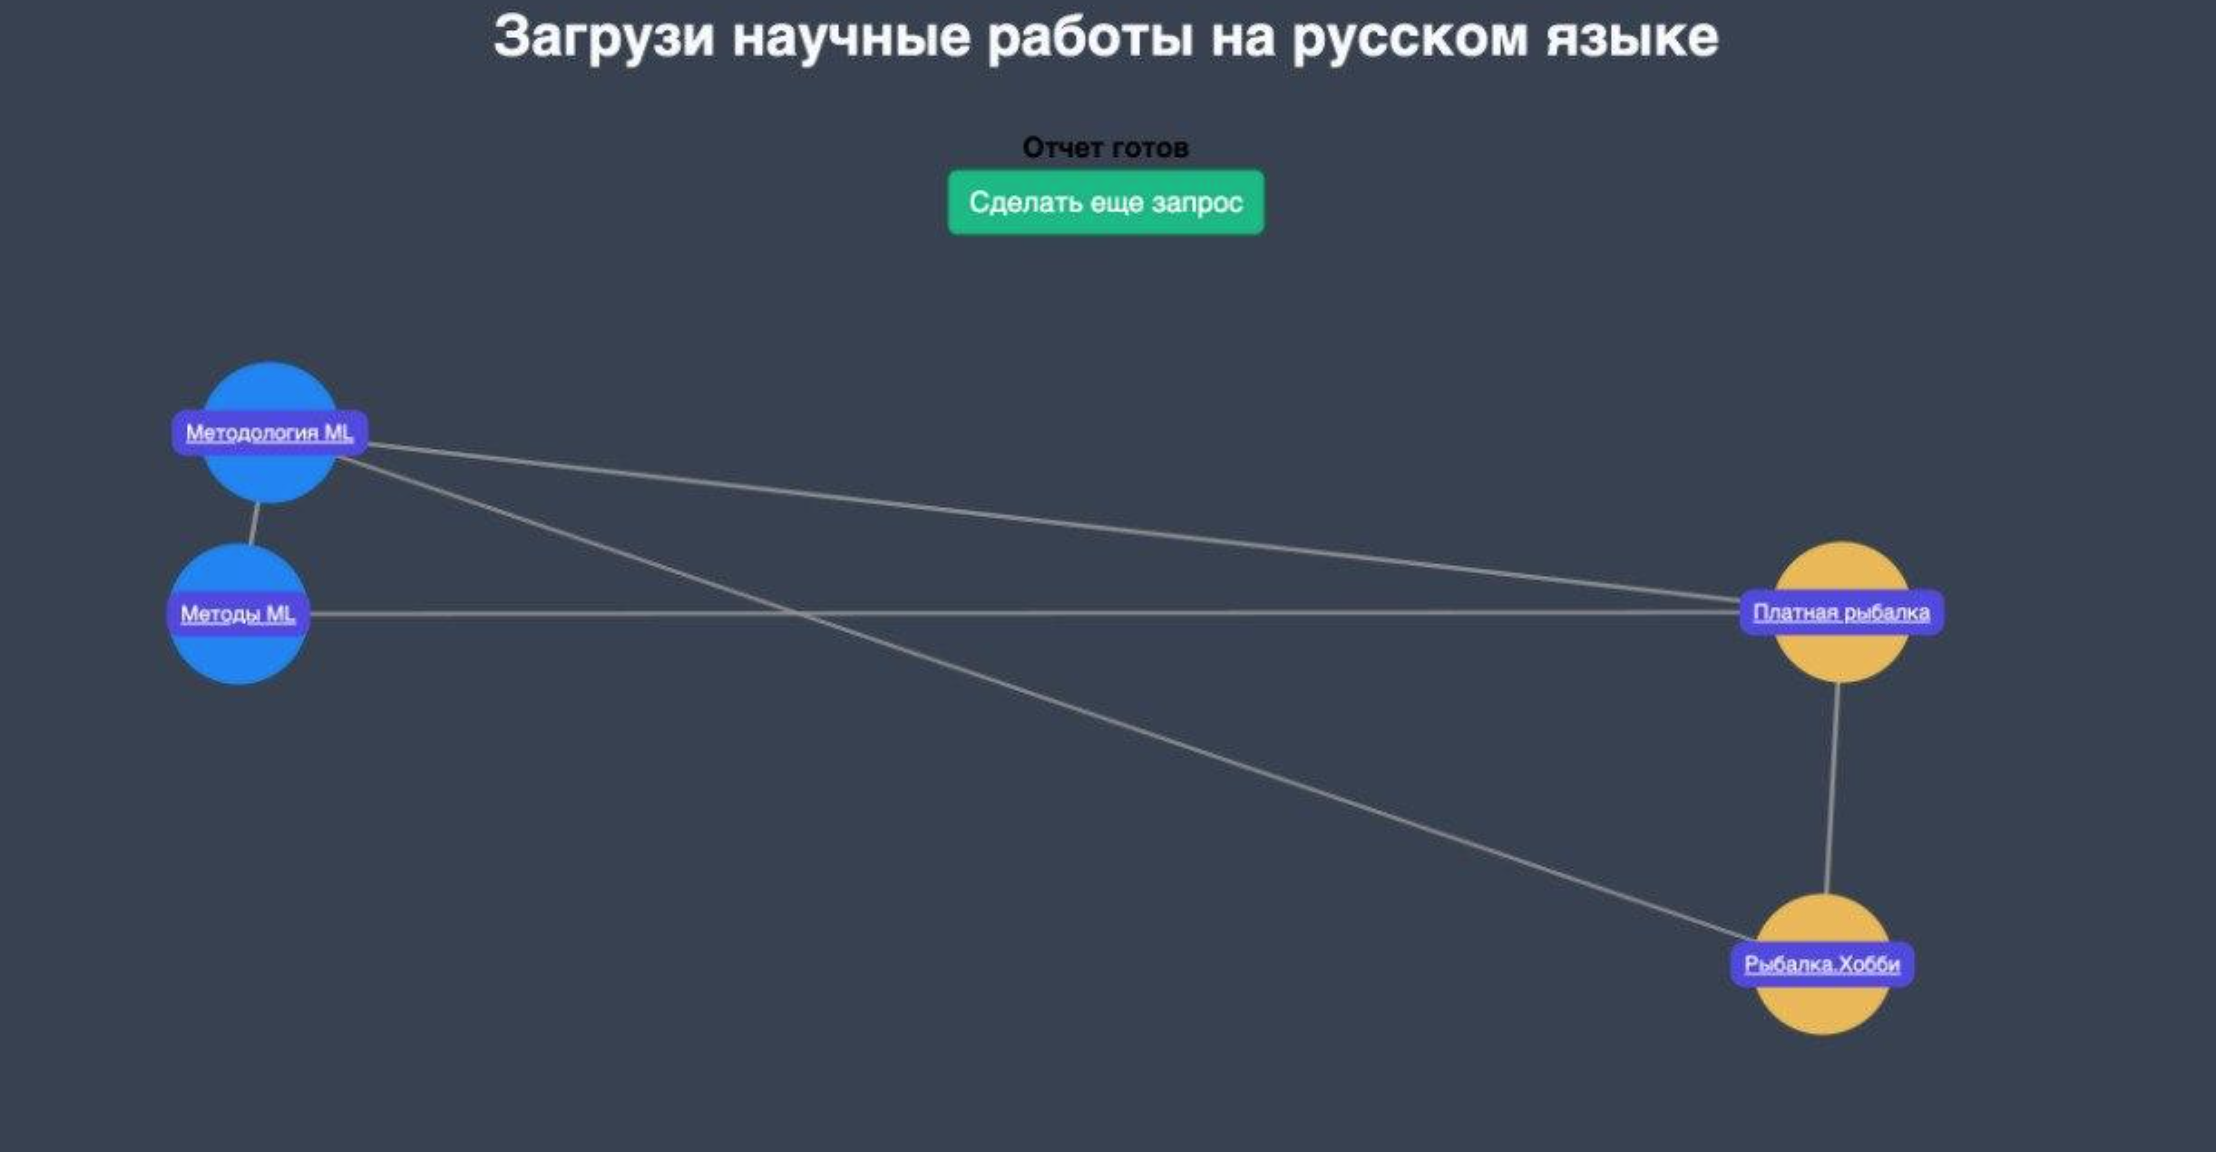
\includegraphics[width=1\textwidth]{styles/diploma/inc/front1.png} 
    \caption{Результат обработки документов}
    \label{fig:example}
\end{figure}  % Теория
\conclusion

 В рамках данной работы была разработана система тематической кластеризации документов, использующая передовые методы семантического анализа и современные алгоритмы машинного обучения. Проведённые тесты и оценка результатов с помощью специализированных метрик подтвердили высокое качество и производительность предложенного решения. Использование микросервисной архитектуры обеспечило необходимую гибкость и масштабируемость, позволяя легко адаптировать систему под различные требования и нагрузки.

Применение модели SBERT-LARGE-NLU-RU и алгоритма кластеризации HDBSCAN продемонстрировало эффективность и высокую точность в задачах обработки и тематического анализа текстовых данных. Интерфейс, представленный в виде графа, обеспечивает удобную визуализацию и простое взаимодействие пользователей с результатами кластеризации.

В дальнейшем планируется совершенствовать систему за счёт расширения функционала, оптимизации алгоритмов обработки данных, улучшения интерфейса и повышения общей производительности. Дополнительным направлением развития может стать интеграция с другими информационными системами и автоматизация процессов мониторинга и анализа больших объёмов текстовых данных.  % Теория


% Теория

%\include{contents/2-01-microservice_architecture}
% \include{contents/2-02.practice}
% \include{contents/2-00-compilation} % Основная часть
% \include{contents/2-01-titlepage}
% \include{contents/2-02-techtask}
% \include{contents/2-03-abstract}
% \include{contents/2-04-glossary}
% \include{contents/9-05-figures}
% \include{contents/2-06-citations}
% \include{contents/2-07-tables}
% \include{contents/2-08-enums}
% \include{contents/2-09-formulas}
% \include{contents/2-10-math}
% \include{contents/2-11-algorithms}
% \include{contents/2-12-listings}
    
\include{contents/3-conclusion} % Заключение

%\printbibliography % Список литературы

\appendix % Приложения
% \include{contents/4-appendix-a}% \include{contents/4-appendix-b}
% \include{contents/4-appendix-c}
% \include{contents/4-appendix-d}
\end{document}
